\chapter{情感} \label{chap:chap42}

兴高采烈、同情、悲伤、恐惧和愤怒通常被认为是情绪的例子。
这些状态对我们的行为和幸福感有着巨大的影响。
但究竟什么是情绪?
区分不同的情绪状态很困难,需要考虑生物体面临的环境或内部产生的挑战及其生理反应。
例如,在我们得出老鼠处于恐惧状态的结论之前,我们需要知道老鼠正在评估特定的威胁刺激(其环境中的捕食者)并且正在做出适应性反应,例如高度唤醒和冻结。


情绪通常沿两个维度表示:效价(即愉快到不愉快)和强度(即低到高唤醒),在许多心理学理论中称为“核心情感”。
然而,情绪也可以分为几类,例如基本情绪类别(快乐、恐惧、愤怒、厌恶、悲伤)和有助于调节社会或道德行为的更复杂情绪类别(例如羞耻、内疚、尴尬、骄傲) ,嫉妒)。
关于是否所有常用类别(如刚才提到的类别)都对应于未来情绪神经科学中科学上有用的类别,存在相当大的争论。


在实验环境中,情绪这个术语有几种不同的使用方式,通常与测量情绪的方式有关(方框 42-1)。
在日常对话中,大多数人将“情绪”一词用作“有意识的情绪体验”或“感觉”的同义词,大多数人类心理学研究也都关注这种“情绪”。
大多数对动物的研究都集中在特定的行为或生理反应上,这在很大程度上是因为在动物研究中不可能获得口头报告。
然而,正如查尔斯·达尔文在他的开创性著作《人与动物的情感表达》中首次观察到的那样,情感在整个物种进化过程中都得到了保护。 因此,我们在本章中描述的实证方法将情绪视为可以在人类和许多其他动物身上研究的中央大脑状态,前提是我们区分情绪和感受。

当大脑检测到某些环境情况时,情绪状态通常会引起广泛的生理反应。 这些生理反应是相对自动的,但取决于环境,并且发生在大脑和全身。 在大脑中,它们涉及唤醒水平和注意力、记忆处理和决策制定等认知功能的变化。 躯体反应涉及内分泌、自主神经和肌肉骨骼系统(第 ~\ref{chap:chap41}~章)。
总之,情绪是神经生物学状态,会引起大脑触发的协调行为和认知反应。
当一个人检测到显着刺激(带正电或带负电)或具有导致内生情绪状态的特定思想或记忆时,就会发生这种情况。


一些刺激物——物体、动物或情境——会触发情绪,而有机体无需学习任何关于这些刺激物的知识。
这种刺激具有先天的强化特性,被称为无条件刺激;
例如痛苦的震惊或恶心的味道。
然而,绝大多数刺激都是通过联想学习获得情感意义的。


当一个人检测到情绪上的重要刺激时,三个生理系统就会参与进来:内分泌腺、自主运动系统和肌肉骨骼系统(图 ~\ref{fig:42_1})。 
内分泌系统负责激素的分泌和调节进入血液,影响身体组织和大脑。
自主神经系统调节身体各种生理控制系统的变化:
心血管系统、内脏器官和体腔组织(第~\ref{chap:chap41}~章)。
骨骼运动系统调节明显的行为,例如冻结、战斗或逃跑以及特定的面部表情。
这三个系统共同控制着身体情绪状态的生理表达。


\begin{figure}[htbp]
	\centering
	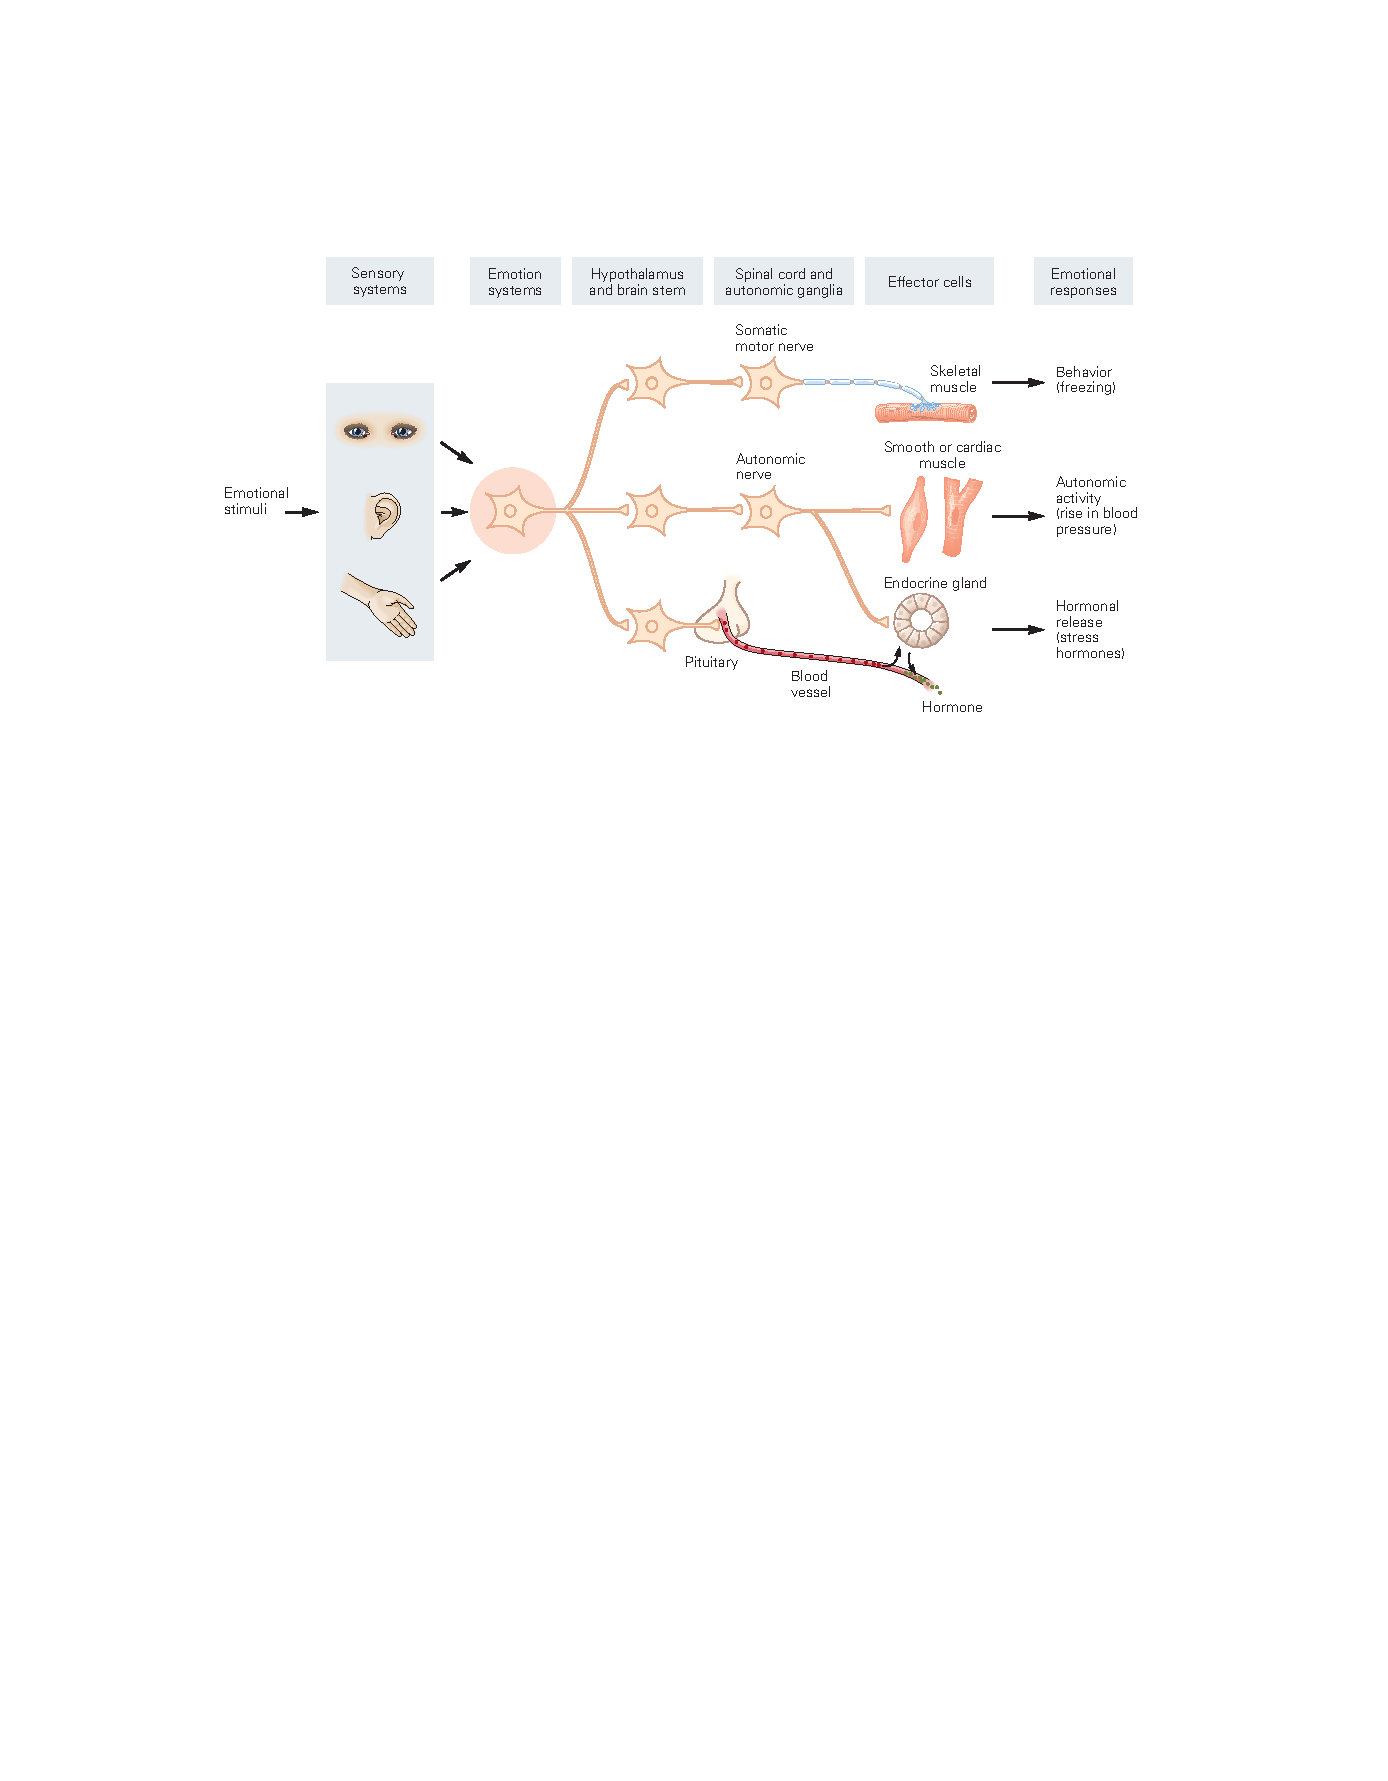
\includegraphics[width=0.8\linewidth]{chap42/fig_42_1}
	\caption{对外部刺激的情绪反应的神经控制。 由感觉系统处理的外部刺激会聚到“情绪系统”(例如,杏仁核)。 如果刺激情绪显着,情绪系统就会被激活,它们的输出会被传递到控制生理反应的下丘脑和脑干区域,包括骨骼肌动作、自主神经系统活动和荷尔蒙释放。 该图显示了一些与恐惧相关的反应。 它忽略了情绪的许多复杂性(例如,情绪状态对认知的影响)。}
	\label{fig:42_1}
\end{figure}


在本章的开头,我们将讨论情绪神经科学现代研究的历史渊源。
然后,我们将描述构成最深入研究的情绪、恐惧的基础的神经回路和细胞机制,在此过程中,我们将重点关注杏仁核。
然而,值得注意的是,似乎没有任何单一的大脑结构只参与一种情绪。
例如,已知参与负价情绪的杏仁核在正价情绪中也起着核心作用:
杏仁核过程中不同的神经元群正价与负价刺激。
我们简要回顾情绪状态如何通过消退和调节而改变,以及情绪如何与其他认知过程相互作用。
最后,我们对情绪研究与理解精神疾病的相关性进行了调查。



\section{对情绪神经回路的现代探索始于 19 世纪末}
现代理解情绪的尝试始于 1890 年,当时美国心理学的创始人威廉·詹姆斯问道:恐惧的本质是什么?
我们是因为害怕而逃离熊,还是因为我们逃跑而害怕?
詹姆斯提出,有意识的恐惧感是逃跑过程中发生的身体变化的结果——我们因为逃跑而感到害怕。
詹姆斯的外围反馈理论借鉴了当时大脑的知识,即大脑皮层有专门负责运动和感觉的区域(图~\ref{fig:42_2})。
当时人们对负责情绪和感觉的大脑特定区域知之甚少,但詹姆斯的观点至今仍在争论不休。


\begin{figure}[htbp]
	\centering
	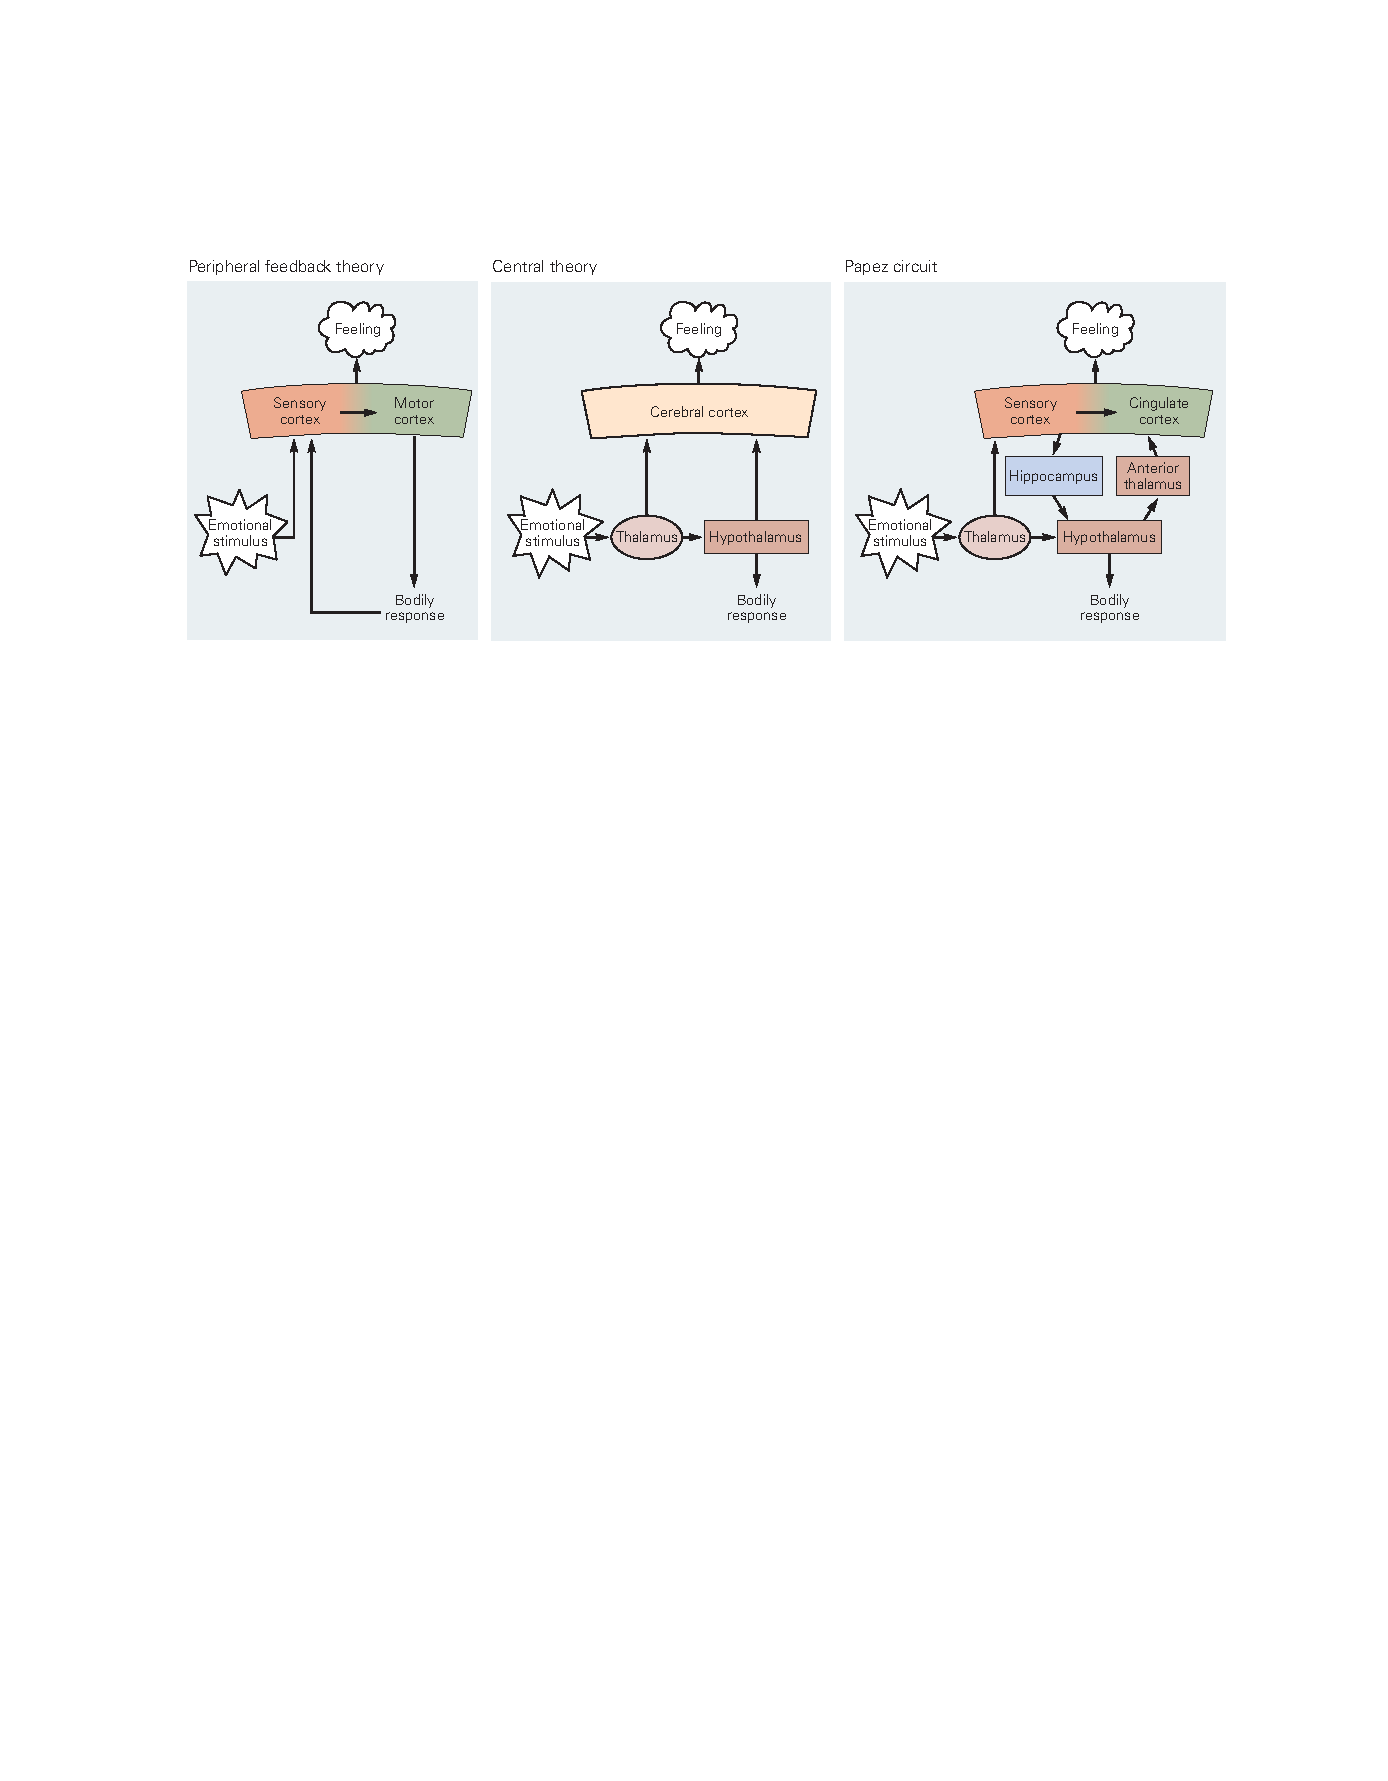
\includegraphics[width=0.95\linewidth]{chap42/fig_42_2}
	\caption{情绪脑的早期理论。(经许可改编自 LeDoux 1996。)William James 的外围反馈理论。 詹姆斯提出,有关情绪能力刺激的信息在感觉系统中进行处理,并传输到运动皮层以在体内产生反应。 到皮层的反馈信号传达有关身体反应的感觉信息。 根据詹姆斯的说法,这种感觉反馈的皮层处理就是“感觉”。 Cannon-Bard 中心理论。 Walter Cannon 和 Philip Bard 提出,情绪是由中枢神经系统内的过程来解释的。 在他们的模型中,感觉信息被传送到丘脑,然后传递到下丘脑和大脑皮层。 下丘脑评估刺激的情绪品质,其与脑干和脊髓的下行连接产生躯体反应,而丘脑皮质通路产生有意识的感觉。 帕佩斯回路。 James Papez 通过添加额外的解剖学特异性改进了 Cannon-Bard 理论。 他提出扣带皮层是在产生感觉时接收下丘脑输出的皮层区域。 下丘脑的输出通过前丘脑到达扣带回,扣带回的输出通过海马体到达下丘脑。}
	\label{fig:42_2}
\end{figure}


在 20 世纪之交,研究人员发现动物在完全切除大脑半球后仍然能够做出情绪反应,这表明情绪的某些方面是由皮层下区域调节的。
下丘脑的电刺激可以引发类似于完整动物情绪反应期间发生的自主反应这一事实向 Walter B. Cannon 暗示,下丘脑可能是控制战或逃反应和其他反应的关键区域。 情绪。


在 1920 年代,Cannon 表明,横断下丘脑水平以上的大脑(通过将皮质、丘脑和下丘脑前部与下丘脑后部和下脑区域分开的切口)留下的动物仍然能够表现出愤怒。
相比之下,下丘脑下方的横断面只留下脑干和脊髓,消除了自然愤怒的协调反应。
这清楚地表明下丘脑参与组织情绪反应。
Cannon 将下丘脑介导的反应称为“虚假愤怒”,因为这些动物缺乏来自皮层区域的输入,他认为这对“真实”愤怒的情绪体验至关重要(图~\ref{fig:42_3})。


\begin{figure}[htbp]
	\centering
	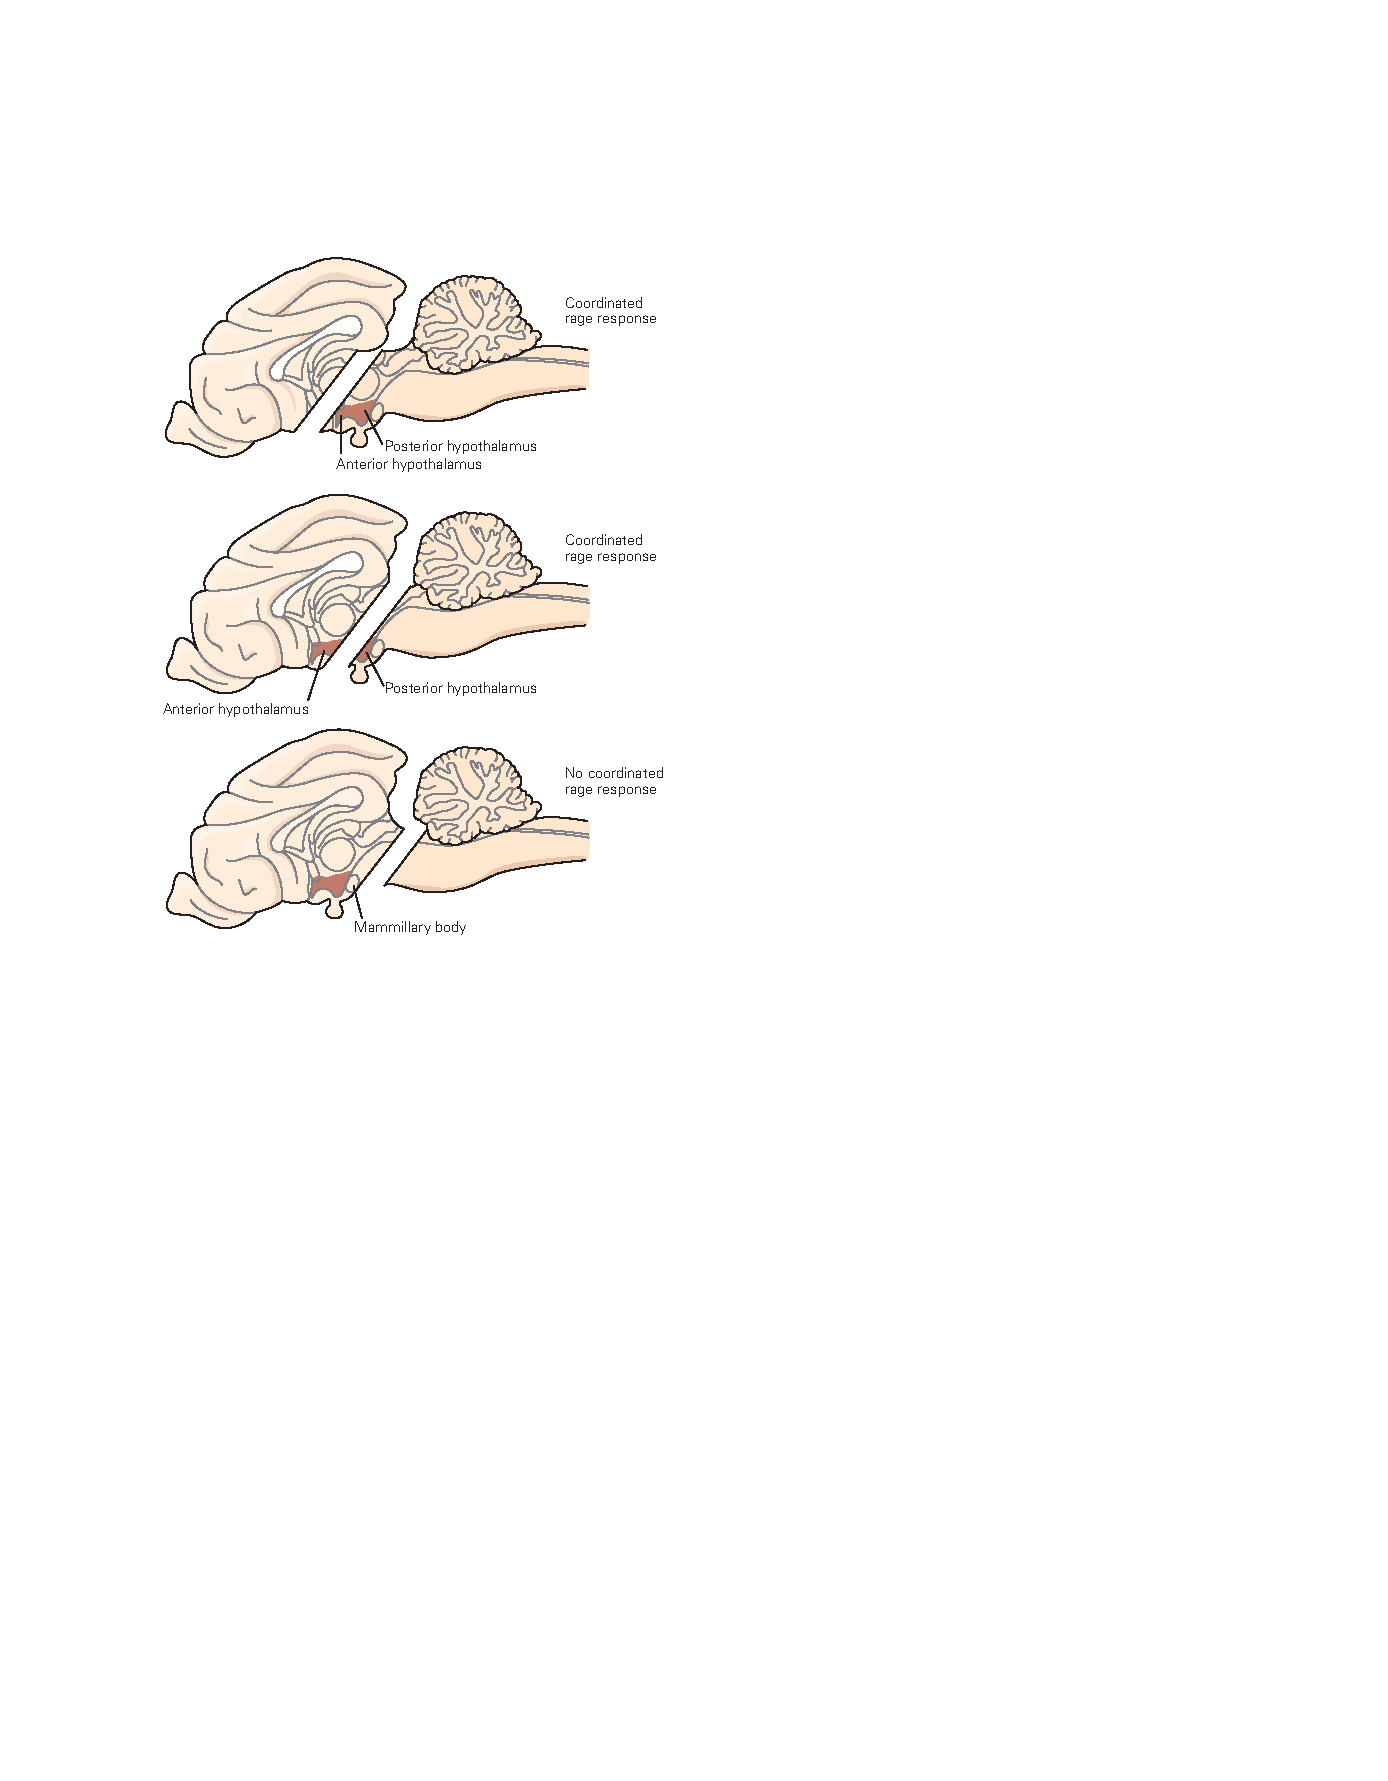
\includegraphics[width=0.5\linewidth]{chap42/fig_42_3}
	\caption{虚假的愤怒。 动物在前脑横断和横断上方的一切(顶部)或前下丘脑水平的横断和它上方的一切断开(中)后表现出虚假的愤怒。 如果下丘脑后部也断开连接(底部),则只能引发孤立的愤怒元素。 这项工作源自动物的历史病变研究。 最近的研究提出了一幅更复杂的图景,其中下丘脑密切参与创造情绪状态本身,而不仅仅是它的行为表达。}
	\label{fig:42_3}
\end{figure}


Cannon 和他的学生 Phillip Bard 提出了一个以下丘脑和丘脑为中心的有影响力的情绪理论。
根据他们的理论,在丘脑中处理的感觉信息被发送到下丘脑和大脑皮层。
对下丘脑的投射被认为会产生情绪反应(通过与脑干和脊髓的连接),而对大脑皮层的投射被认为会产生有意识的感觉(图~\ref{fig:42_2})。
该理论暗示下丘脑负责大脑评估外部刺激的情绪意义,情绪反应取决于这种评估。


1937 年,James Papez 扩展了 Cannon-Bard 理论。 与 Cannon 和 Bard 一样,Papez 提出来自丘脑的感觉信息被发送到下丘脑和大脑皮层。
与脑干和脊髓的下行连接产生情绪反应,与大脑皮层的上行连接产生感觉。
但是,帕佩兹通过在下丘脑和大脑皮层之间插入一组新结构,进一步扩展了感觉的神经回路,远远超出了 Cannon-Bard 理论。
他认为来自下丘脑的信号首先到达前丘脑,然后到达扣带皮层,来自下丘脑和感觉皮层的信号会聚在这里。
这种融合解释了帕佩斯理论中有意识的感觉体验。
感觉皮层然后投射到扣带皮层和海马体,后者又与下丘脑的乳头体连接,从而完成环路(图~\ref{fig:42_2})。


下丘脑目前受到动物情绪研究的浓厚兴趣,特别是在使用光遗传学操纵精确细胞群活动的实验中。
这些研究表明,小鼠腹内侧下丘脑中的特定群体对于防御性情绪状态是必要且充分的。
因此,下丘脑不仅协调情绪行为,而且是构成情绪状态本身的神经回路的一部分。
下丘脑在情绪中的作用在人类中的研究要少得多,部分原因是功能性磁共振成像没有空间分辨率来研究特定的下丘脑核,更不用说其中的神经元亚群了。


1930 年代后期,海因里希·克卢弗 (Heinrich Klüver) 和保罗·布西 (Paul Bucy) 切除了猴子的双侧颞叶,从而损害了所有颞叶皮层以及杏仁核和海马体等皮质下结构,并发现了各种心理障碍,包括进食习惯的改变(猴子 把不能吃的东西放进嘴里)和性行为(他们试图与不合适的伴侣发生性关系,比如其他物种的成员)。
此外,猴子对以前害怕的物体(例如,人和蛇)明显缺乏关注。
这组非凡的发现后来被称为 Klüver-Bucy 综合症,并且已经表明杏仁核可能对情绪很重要(尽管它不是这些实验中唯一受损的结构)。


基于 Cannon-Bard 和 Papez 模型以及 Klüver 和 Bucy 的发现,Paul MacLean 在 1950 年提出情绪是“内脏大脑”的产物。
根据 MacLean 的说法,内脏脑包括各种皮质区域,这些区域长期以来被称为边缘叶,保罗布罗卡之所以这样命名,是因为这些区域在半球的内侧壁形成一个边缘(拉丁语边缘)。
内脏脑后来改名为边缘系统。 边缘系统包括构成布罗卡边缘叶的各种皮质区域(尤其是颞叶和额叶的内侧区域)以及与这些皮质区域相连的皮层下区域,例如杏仁核和下丘脑(图~\ref{fig:42_4})。


\begin{figure}[htbp]
	\centering
	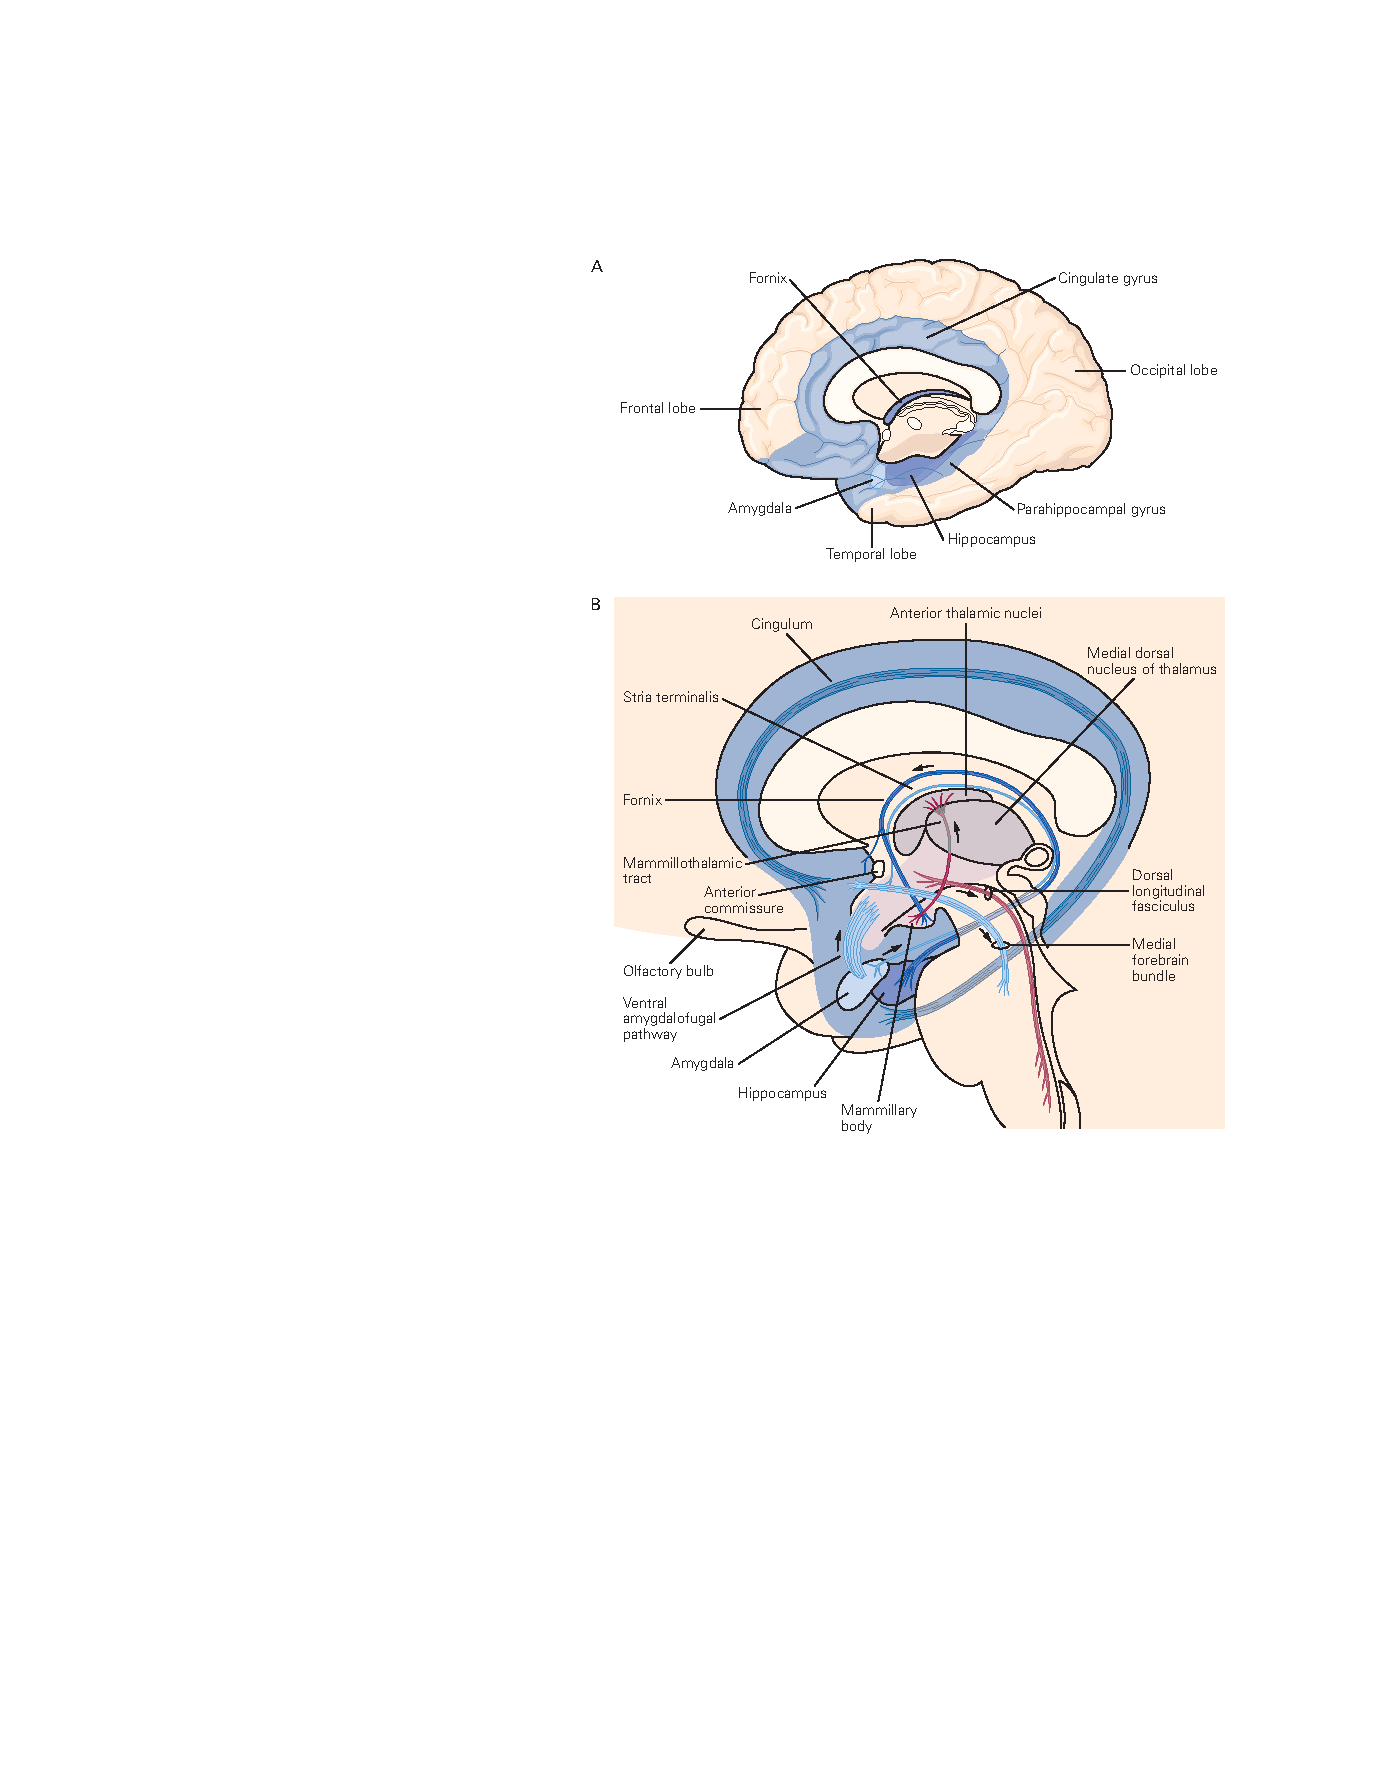
\includegraphics[width=0.6\linewidth]{chap42/fig_42_4}
	\caption{边缘系统由边缘叶和深层结构组成。 (经许可改编自 Nieuwenhuys 等人,1988 年。) A. 这张大脑的内侧视图显示了前额叶边缘皮层和边缘叶。 边缘叶由环绕上脑干的原始皮质组织(蓝色)以及下方的皮质结构(海马体和杏仁核)组成。 B. 边缘系统中深层结构的互连。 箭头表示每个束中神经活动的主要方向,尽管这些束通常是双向的。}
	\label{fig:42_4}
\end{figure}


麦克莱恩打算将他的理论作为对帕佩斯思想的详尽阐述。
事实上,麦克莱恩边缘系统的许多区域都是帕佩斯回路的一部分。
然而,麦克莱恩并不赞同帕佩斯关于扣带皮层是感觉所在的观点。
相反,他认为海马体是大脑的一部分,外部世界(代表在外侧皮层的感觉区域)与内部世界(代表在内侧皮层和下丘脑)汇聚在一起,允许内部信号赋予情绪权重 外部刺激,从而产生有意识的感觉。
对于麦克莱恩来说,海马体既参与身体情绪反应的表达,也参与有意识的感受体验。


随后的发现为麦克莱恩的边缘系统理论提出了问题。 1957 年,人们发现海马体(边缘系统的基石)受损会导致短期记忆向长期记忆的转化出现缺陷,而这种功能不同于情绪。
此外,海马体受损的动物能够表达情绪,而海马体受损的人似乎可以正常表达和感受情绪。
一般来说,边缘系统区域的损伤不会对情绪行为产生预期的影响。


尽管如此,麦克莱恩关于情感的其他一些观点仍然具有现实意义。
MacLean 认为情绪反应对生存至关重要,因此涉及在进化过程中保存下来的相对原始的回路,这一观点早在近一个世纪前就已由 Charles Darwin 提出。
这个概念是情感进化观点的关键。
现在很清楚,情绪是由许多皮层下和皮层区域处理的,边缘系统绝不是情绪的主要系统。
尽管如此,杏仁核是原始边缘系统的一个组成部分,在人类和动物研究中受到的关注最多。
今天,杏仁核在习得性恐惧中的作用可能是特定大脑结构中情绪处理的最佳例子,因此,我们接下来会考虑它。



\section{杏仁核与后天恐惧和先天恐惧有关}

在巴甫洛夫恐惧条件反射中,学习了无条件刺激 (US)(例如电击)和预测美国的条件刺激 (CS)(例如音调)之间的关联。
例如,如果给动物呈现几秒钟的情绪中性 CS(音调),然后在 CS 的最后一秒受到电击,特别是如果这种音调和电击配对重复多次,仅呈现音调就会 引发防御性冻结以及自主神经和内分泌活动的相关变化。
此外,许多防御性反应,例如眨眼和吃惊,仅通过语气就会得到促进。


许多实验室的研究表明,杏仁核是巴甫洛夫恐惧条件反射所必需的:
杏仁核受损的动物无法学习 CS 与 US 之间的关联,因此当 CS 稍后单独呈现时不会表达恐惧。


杏仁核由大约 12 个核组成,但侧核和中央核在恐惧条件反射中尤为重要(图~\ref{fig:42_5})。
对任一核的损伤,而不是对其他区域的损伤,可以防止恐惧条件反射。
杏仁核的外侧核接收大部分感觉输入(但内侧核接收嗅觉输入),包括来自丘脑和皮层的关于 CS 的感觉信息(例如,音调)。
已经详细阐明了杏仁核内构成习得性恐惧的细胞和分子机制,尤其是在侧核中。
这些发现支持了这样一种观点,即侧核是恐惧条件反射中的记忆存储部位。
相比之下,中央核中的神经元将输出调解到涉及防御行为控制和相关自主神经和体液反应的脑干区域(第~\ref{chap:chap41}~章)。
侧核和中央核通过杏仁核内的几个局部环路连接,包括与基底块和层间块的连接。
因此,巴甫洛夫学习的实际回路比图~\ref{fig:42_5}~所示的要复杂得多,涉及杏仁核区域之间的多个中继。


\begin{figure}[htbp]
	\centering
	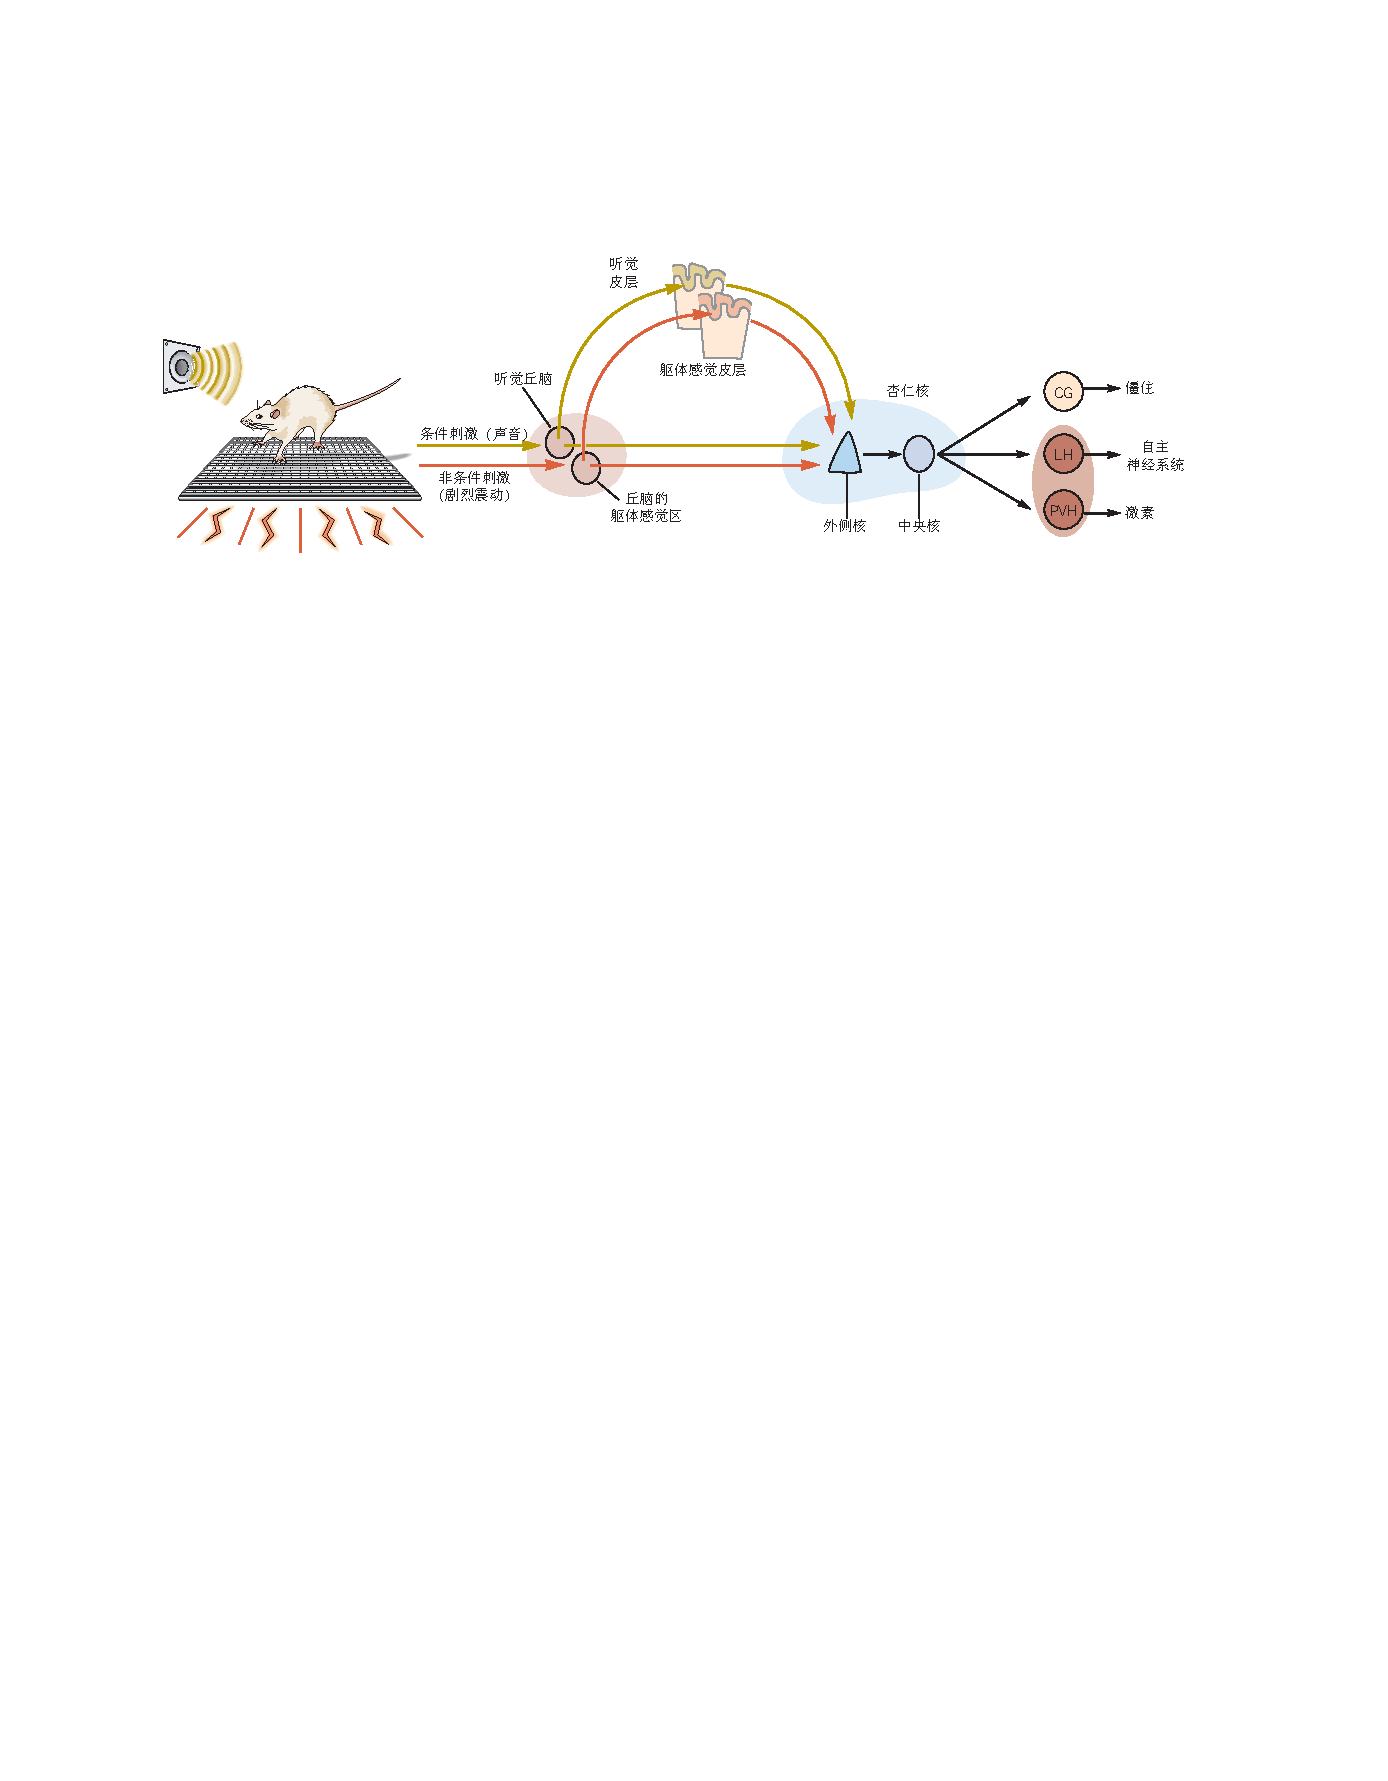
\includegraphics[width=0.95\linewidth]{chap42/fig_42_5}
	\caption{神经回路在恐惧条件反射期间参与。条件刺激 (CS) 和非条件刺激 (US) 从丘脑和大脑皮层的听觉和体感区域传递到杏仁核的外侧核。 CS 和 US 通路在侧核中的融合被认为是介导学习的突触变化的基础。 外侧核直接和通过涉及基底核和嵌入核的杏仁核内通路(未显示)与中央核相通。 中央核将这些信号传递到控制各种运动反应的区域,包括控制冻结行为的中央灰色区域 (CG); 控制自主反应的外侧下丘脑 (LH); 和室旁下丘脑 (PVH),它通过垂体-肾上腺轴控制应激激素的分泌。 (改编自 Medina 等人,2002 年。)}
	\label{fig:42_5}
\end{figure}


感觉输入直接和间接地从丘脑到达外侧核。
正如 Cannon-Bard 假说所预测的那样,来自丘脑中继核的感觉信号被传送到大脑皮层的感觉区域。
结果,杏仁核和皮层同时被激活。
然而,杏仁核能够在皮层完全处理刺激信息之前对听觉危险提示做出反应。
该方案仅适用于啮齿动物的听觉恐惧条件反射,目前尚不清楚它如何应用于其他情况,例如人类视觉诱发的恐惧。


侧核被认为是恐惧调节过程中突触变化的部位。
CS 和 US 信号集中在侧核的神经元上;
当 CS 和 US 配对时,CS 在引发动作电位方面的有效性得到增强。
这种联想学习形式的基本机制类似于海马体中陈述性记忆的细胞机制(第~\ref{chap:chap54}~章)。
特别是,海马体中发现的突触可塑性也在特定的中央杏仁核回路中得到证实。
因此,中央杏仁核不仅驱动电机输出,而且还是形成和存储恐惧关联的回路的一部分,很可能是通过从侧核传输有关 CS 和 US 的信息。
在恐惧学习过程中,神经可塑性也可能发生在基底核和副基底核中。
与下丘脑一样,最近在啮齿动物中使用光遗传学等工具来操纵杏仁核神经元的特定亚群的研究已经开始更详细地剖析该回路。


杏仁核与其他大脑结构(例如前额叶皮层)一起评估刺激的情绪变化。
如果该系统检测到危险,它会通过从中央杏仁核和部分前额叶皮层到下丘脑和脑干的连接来协调行为和生理反应的表达。
例如,冻结行为是由中央核与腹侧导水管周围灰色区域的连接介导的。
此外,杏仁核的基底核和辅助基底核向大脑皮层的许多部分发送投射,包括前额叶、鼻腔和感觉皮层;
这些通路为杏仁核中的神经表征提供了一种影响认知功能的方法。
例如,通过广泛投射到皮层区域,杏仁核可以调节注意力、知觉、记忆和决策制定。
它与投射到皮层区域的调节性多巴胺能、去甲肾上腺素能、血清素能和胆碱能核的联系也影响认知过程(第~\ref{chap:chap40}~章)。
鉴于这些非常广泛的联系和功能影响,杏仁核非常适合实现情绪的关键特征之一:协调和多组分反应。



\subsection{杏仁核与动物天生的恐惧有关}

虽然大多数刺激通过学习获得情感意义,尤其是在人类中,但许多动物也依赖于先天(无条件)信号来检测威胁、配偶、食物等。
例如,当检测到狐狸尿液时,啮齿动物会表现出冻结和其他防御行为。
最近的研究在揭示这种先天恐惧背后的回路方面取得了相当大的进展。


在哺乳动物中,涉及捕食者或同种气味的无条件威胁的感觉信号从嗅觉系统的犁鼻部分(第~\ref{chap:chap29}~章)传输到内侧杏仁核。
这与听觉和视觉威胁形成对比,如上所述,听觉和视觉威胁是通过外侧杏仁核处理的。
内侧杏仁核的输出到达与下丘脑前乳头核相连的腹内侧下丘脑。
与依赖于腹侧导水管周围灰色区域的习得性恐惧相反,无条件的恐惧反应取决于从下丘脑到背侧导水管周围灰色区域的输入。
还有其他专门用于处理特定先天威胁的皮层下系统;
例如,老鼠的上丘参与检测空中捕食者,例如从头顶飞过的鹰。


很难研究人类无条件的情绪反应,因为学习的可能性从出生就开始,无法通过实验控制,而且个体差异似乎很大。
例如,对于那些对这些动物有恐惧症的人,人们认为蛇和蜘蛛等与威胁相关的刺激可能是天生的恐惧诱发刺激,但对于将它们作为宠物饲养的人来说则不然。
这些巨大的个体差异,以及先天恐惧和习得恐惧的相对作用,是理解焦虑症等精神疾病的重要主题。



\subsection{杏仁核对人类的恐惧很重要}

动物研究中关于杏仁核在情绪中的作用的基本发现已在人类研究中得到证实。
杏仁核受损的患者在中性 CS 与 US(电击或巨响)配对时无法表现出恐惧条件反射。
在正常人类受试者中,杏仁核的活动在 CS-US 配对期间增加,如用\textit{功能性磁共振成像}测量的那样。


对患有双侧杏仁核损伤的罕见人类患者的研究导致了令人惊讶的发现,即对外部感受和内部感受刺激的恐惧反应分离(图~\ref{fig:42_6})。
这些患者不仅对 CS 或 US 的外部感受性刺激没有表现出任何自主恐惧反应,而且他们似乎也缺乏任何有意识的恐惧体验,这从行为观察或通过问卷中的主观口头报告得到证明。
在一项研究中,这样的患者在异国情调的宠物店里遇到了蛇和蜘蛛,在鬼屋里遇到了怪物,并且对高度创伤性的个人事件(例如,受到另一个人的死亡威胁)进行了自传式回忆。
在这些情况下,没有任何恐惧的迹象,患者报告说根本没有感到恐惧(即使患者能够感受到其他情绪)。
这些发现表明,杏仁核对于人类恐惧的诱发和体验是必不可少的。


\begin{figure}[htbp]
	\centering
	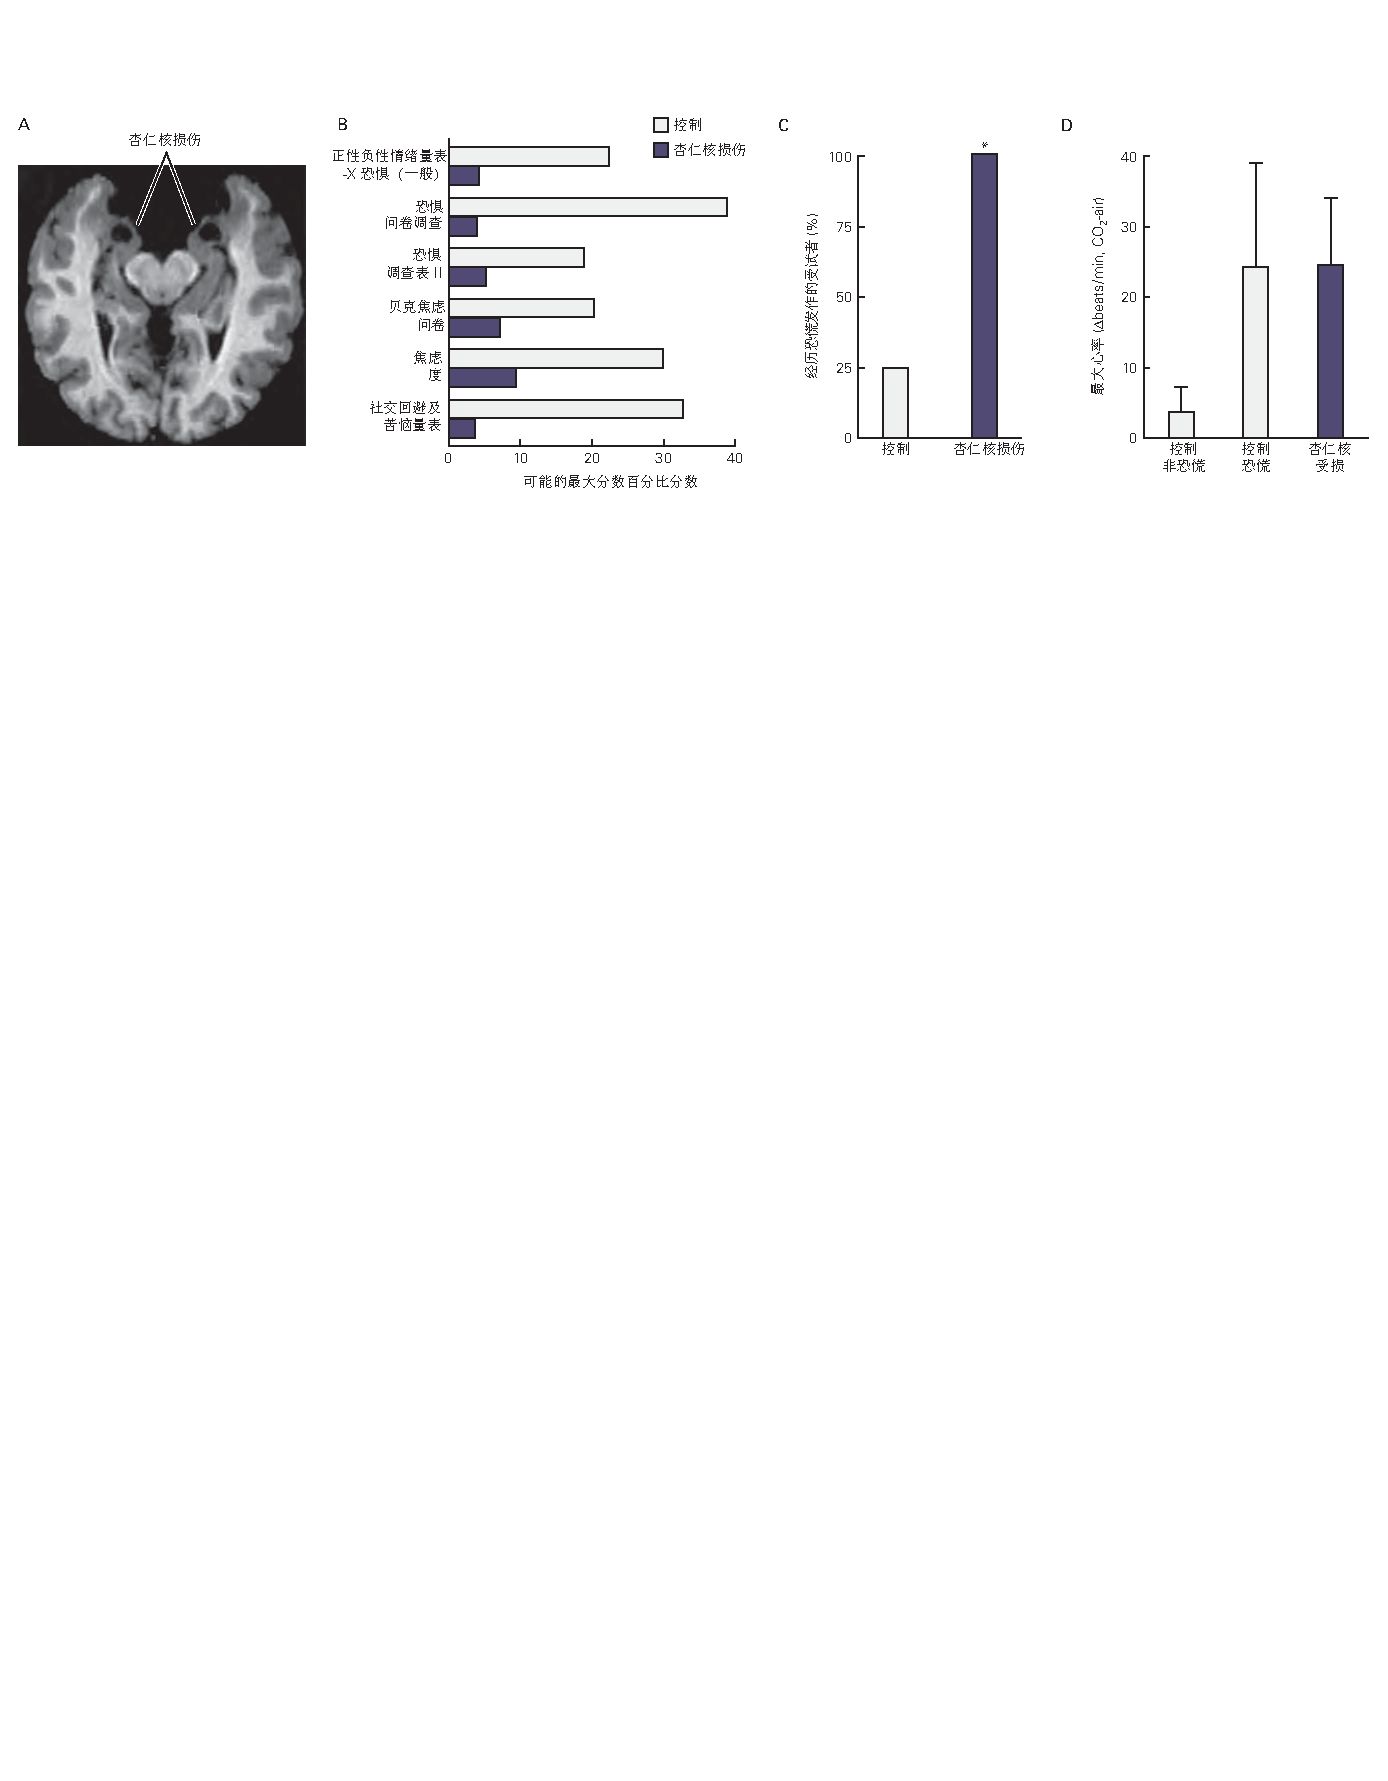
\includegraphics[width=0.7\linewidth]{chap42/fig_42_6}
	\caption{在人类中,杏仁核对于对外部而非内部刺激的恐惧反应是必需的。 A. 双侧杏仁核损伤受试者大脑的磁共振成像扫描。 病变相对局限于整个杏仁核,这在人类中是非常罕见的病变。 B. 患有双侧杏仁核损伤的受试者 S.M. 没有报告对通常用于评估恐惧和焦虑的任何基于问卷的措施感到恐惧(可能的最大分数百分比 [POMP])。 这与其他调查结果一致:她在看恐怖电影、面对大型蜘蛛和蛇或在万圣节期间参观鬼屋时没有表现出恐惧。 这些发现表明,人类杏仁核对于诱发对这些外部刺激做出反应的恐惧是必不可少的。 (缩写:PANAS,Positive and Negative Affect Schedule。)C. 相比之下,对 S.M. 的研究 和另外两名患有双侧杏仁核损伤的受试者发现,当受到内部刺激时,他们表现出强烈的恐慌。 他们被要求吸入二氧化碳 (CO2),这会产生窒息感。 这导致所有 3 名杏仁核受损患者和 12 名杏仁核完整的对照组中的 3 名出现惊恐发作。 D. 相对于空中试验,吸入 CO2 期间最大心率相对于基线的变化。 杏仁核损伤患者 (n = 2) 和惊慌失措的对照组 (n = 3) 的心率增幅均高于未惊慌的对照组 (n = 9)。 (平均值 ± 平均值的标准误差。)(改编自 Feinstein 等人 2011 年、2013 年的许可。)}
	\label{fig:42_6}
\end{figure}


与此形成鲜明对比的是,同样患有杏仁核损伤的患者在感到自己好像快要窒息时会表现出强烈的恐慌(一种内感受性恐惧线索,通过吸入二氧化碳来降低血液 pH 值)。
恐惧反应对外感受和内感受刺激的分离支持了这样一种观点,即人脑中存在多种恐惧系统,杏仁核不可能是所有形式恐惧的唯一必要结构。
正在进行的工作正在提供更多的见解,例如绘制出这些患者受损的特定杏仁核,以及哪些核对哪些类型的缺陷负责。
这种水平的分辨率在杏仁核的动物研究中是标准的,但在人类中很难达到,因为杏仁核损伤不能通过实验进行,而必须依赖于反映自然事故的罕见患者。
同样重要的是,对于如何细分不同类型的恐惧,存在理论框架。
例如,恐惧可以映射到威胁迫在眉睫的维度上,它可能涵盖从非常遥远的威胁(可能引起轻微的焦虑,并参与监控和关注)到更近的威胁(引起恐惧,以及 参与反应,如冻结),对即将导致死亡的威胁(引起恐慌,并参与防御行为)。
最终,我们需要在大脑系统和包含所有这些细节的各种情绪之间建立更精细的映射。


某些形式的恐惧学习对人类来说是相对独特的。
例如,简单地告诉人类受试者 CS 之后可能会受到电击就足以让 CS 引发恐惧反应。
CS 会引发特征性的自主反应,即使它从未与电击的传递相关联。
人类也可以通过允许他们观察其他被制约的人来制约——观察者学会害怕 CS,即使 CS 或 US 从未直接呈现给观察对象。
其他一些动物也能够通过这种观察学习来学习恐惧,尽管这种情况似乎比人类更为罕见。
一种在人类中普遍存在的学习形式似乎是我们物种独有的:主动教学法,即另一个人教另一个人一种刺激是危险的。
虽然学习在世界上应该避免什么和应该接近什么是所有物种幼崽发展的重要组成部分,但迄今为止,除了人类以外的任何物种都没有发现关于刺激重要性的主动教学(通过被动观察学习是 比较普遍;普遍上)。


人类杏仁核的情绪学习和记忆能力属于内隐学习和记忆的范畴,其中包括记忆的形式,例如感知和运动技能的无意识回忆(第~\ref{chap:chap53}~章)。
然而,在危险情况下,参与外显学习和记忆(对人、地点和事物的有意识回忆)的海马体和内侧颞叶系统的其他组成部分也会被招募,并将对学习事件的各个方面进行编码 。
因此,学习到的危险指标也可以有意识地回忆起来,至少在人类中,可能在其他一些物种中也是如此。


对杏仁核或海马双侧损伤患者的研究表明,这些结构分别对情绪事件的内隐记忆和外显记忆有不同的贡献。
杏仁核受损的患者对 CS 没有条件性皮肤电导反应(表明没有内隐情绪学习),但对调节体验有正常的陈述性记忆(表明完整的外显学习)。
相比之下,海马损伤患者对 CS 表现出正常的条件性皮肤电导反应(表明完整的内隐情绪学习),但对条件反射体验没有自觉记忆(表明外显学习受损)。


杏仁核功能在人类的许多精神疾病中发生了改变,尤其是恐惧和焦虑症(第~\ref{chap:chap51}~章)。
此外,杏仁核在处理与成瘾药物相关的线索中起着重要作用(第~\ref{chap:chap43}~章)。
在所有这些情况下,杏仁核只是包括其他皮层和皮层下区域的分布式神经网络的一个组成部分。
例如,对高度情绪化事件的陈述性记忆涉及杏仁核和海马体之间的相互作用;
巴甫洛夫条件反射的动机后果涉及杏仁核和腹侧纹状体之间的相互作用;
了解以前危险的刺激现在是安全的涉及杏仁核和前额叶皮层之间的相互作用。
一个重要的未来方向将是超越孤立地检查每个组件,以便更好地了解复杂的大脑区域多组件网络如何处理情绪。
这种分析水平在使用\textit{功能性磁共振成像}的人类情感研究中很常见(见下文)。



\subsection{杏仁核的作用延伸到积极情绪}

虽然在过去半个世纪中,大多数关于情绪神经基础的工作都集中在厌恶反应上,尤其是恐惧,但其他研究表明,杏仁核也参与积极情绪,特别是奖励的处理。
在猴子和啮齿动物中,杏仁核参与将中性刺激与奖励(食欲巴甫洛夫条件反射)联系起来,就像它参与将中性刺激与惩罚联系起来一样,并且在杏仁核中似乎有不同的神经元群编码奖励和惩罚。
这与啮齿动物下丘脑的发现大致相似,其中参与防御和交配的神经元也靠得很近,只有现代分子技术才能测试它们的独立作用。


对非人类灵长类动物和啮齿动物的研究调查了 Larry Weiskrantz 首先提出的一个建议,即杏仁核代表刺激奖赏和惩罚。
例如,在最近的一项研究中,猴子被训练将抽象的视觉图像与奖励或厌恶的 US 联系起来。
然后含义被颠倒(例如,通过将厌恶结果与先前与奖励相关联的视觉图像配对)。
通过这种方式,可以区分杏仁核在表示视觉信息中的作用与其在表示视觉图像预测的强化(奖励或厌恶刺激)中的作用。
与图像相关的强化类型的变化调节了杏仁核中的神经活动,并且调节发生得足够快以解释行为学习。


随后使用现代分子和遗传技术的研究表明,杏仁核内的不同回路介导了奖励性 US 以及奖励性体验的神经表征。
杏仁核中食欲 US 的神经表征的激活足以诱导先天性生理反应以及食欲学习。
此外,先前被愉快体验激活的神经元的再激活似乎足以引发积极情绪。
这些发现与越来越多的人类功能成像研究一致,这些研究表明杏仁核相当广泛地参与情绪。
例如,当受试者观察到与食物、性和金钱相关的刺激图片时,或者当人们根据刺激的奖励价值做出决定时,人类杏仁核就会被激活。



\section{情绪反应可以通过消退和调节来更新}

一旦习得了条件性恐惧,就可以通过稍后体验 CS 现在是安全的来消除它,例如,在没有任何 US 配对的情况下反复呈现 CS。
恐惧消退的潜在回路已被详细研究,因为它与创伤后应激障碍 (PTSD) 等精神疾病高度相关。
需要从前额叶皮层到杏仁核的投射来克服杏仁核中的条件性恐惧。
虽然有条件的恐惧反应在灭绝期间会下降,但它们永远不会被完全消除,正如恢复现象所证明的那样,恐惧会突然重新出现。


还研究了用于改变情绪状态的认知疗法,主要是在人类中。
例如,集中精力增加或减少恐惧等情绪的强度会对情绪状态产生一些影响。
事实上,神经影像学研究发现,在某种程度上,人们可以通过他们对这些刺激的思考方式将他们的杏仁核激活改变为引起恐惧的刺激。
情绪调节是一种复杂的现象,因为有多种策略可以改变情绪,从仅仅抑制运动行为到更好地控制我们如何评估情况。
这些情绪调节的多种来源,尤其是在人类中,突出了一个事实,即必须经常调整情绪以与复杂的社会规范保持一致。



\section{情绪会影响认知过程}

如以上示例所示,情绪与认知的许多其他方面相互作用,包括记忆、决策和注意力。
我们在上面讨论了一个非陈述性情绪记忆的例子,即巴甫洛夫恐惧条件反射,但情绪也会影响陈述性记忆。
从杏仁核到海马体的投射可以影响学习如何编码和巩固到长期陈述性记忆中。
这就是为什么我们对生活中最情绪化的事件记忆最深刻的原因,例如婚礼和葬礼。


正如人们所预料的那样,情绪对决策制定具有复杂的影响,因为风险、努力和价值等变量的主观评估受情绪调节。
例如,具有相同客观风险的不同选择可能会引发不同的行为决策,具体取决于它们是赢还是输。
例如,受试者通常更喜欢确定获得 5 美元而不是有 50\% 的机会赢得 10 美元,但更喜欢有 50\% 的机会损失 10 美元而不是确定损失 5 美元。
有趣的是,\textit{功能性磁共振成像}研究表明,这种框架可以调节杏仁核的激活。
当受试者选择一定金额而不是冒险赌博时,“赢”框架中的杏仁核会更加活跃,而当受试者选择赌博而不是确定金额时,“失败”框架中的杏仁核会更加活跃。
因此,杏仁核中的价值表征并不严格与刺激相关,而是受上下文相关评估的调节。


因为与情感相关的刺激对有机体的自身利益非常重要,所以它们通常会引起注意。
例如,人们倾向于定向和注视与情感相关的视觉刺激,即使这些刺激是在无法有意识地感知的情况下呈现的。
一个有趣的发现是,患有双侧杏仁核损伤的患者不仅在恐惧的体验和表达上受损,如上所述,而且在他们对他人恐惧的认识上也受损。
一位这样的患者,一位名叫 S.M. 的女性,在从面部表情识别恐惧方面有选择性地受损。
这种损伤反过来似乎是由于将视觉注意力分配到通常表示恐惧的面部区域的更基本的损伤。
S.M. 当她看面部表情时,她不会自发地注视面部的眼睛区域,因此不会处理来自睁大眼睛的详细视觉信息,而这些信息通常有助于在一个人看一张恐惧的脸时识别恐惧(图~\ref{fig:42_7}))。


\begin{figure}[htbp]
	\centering
	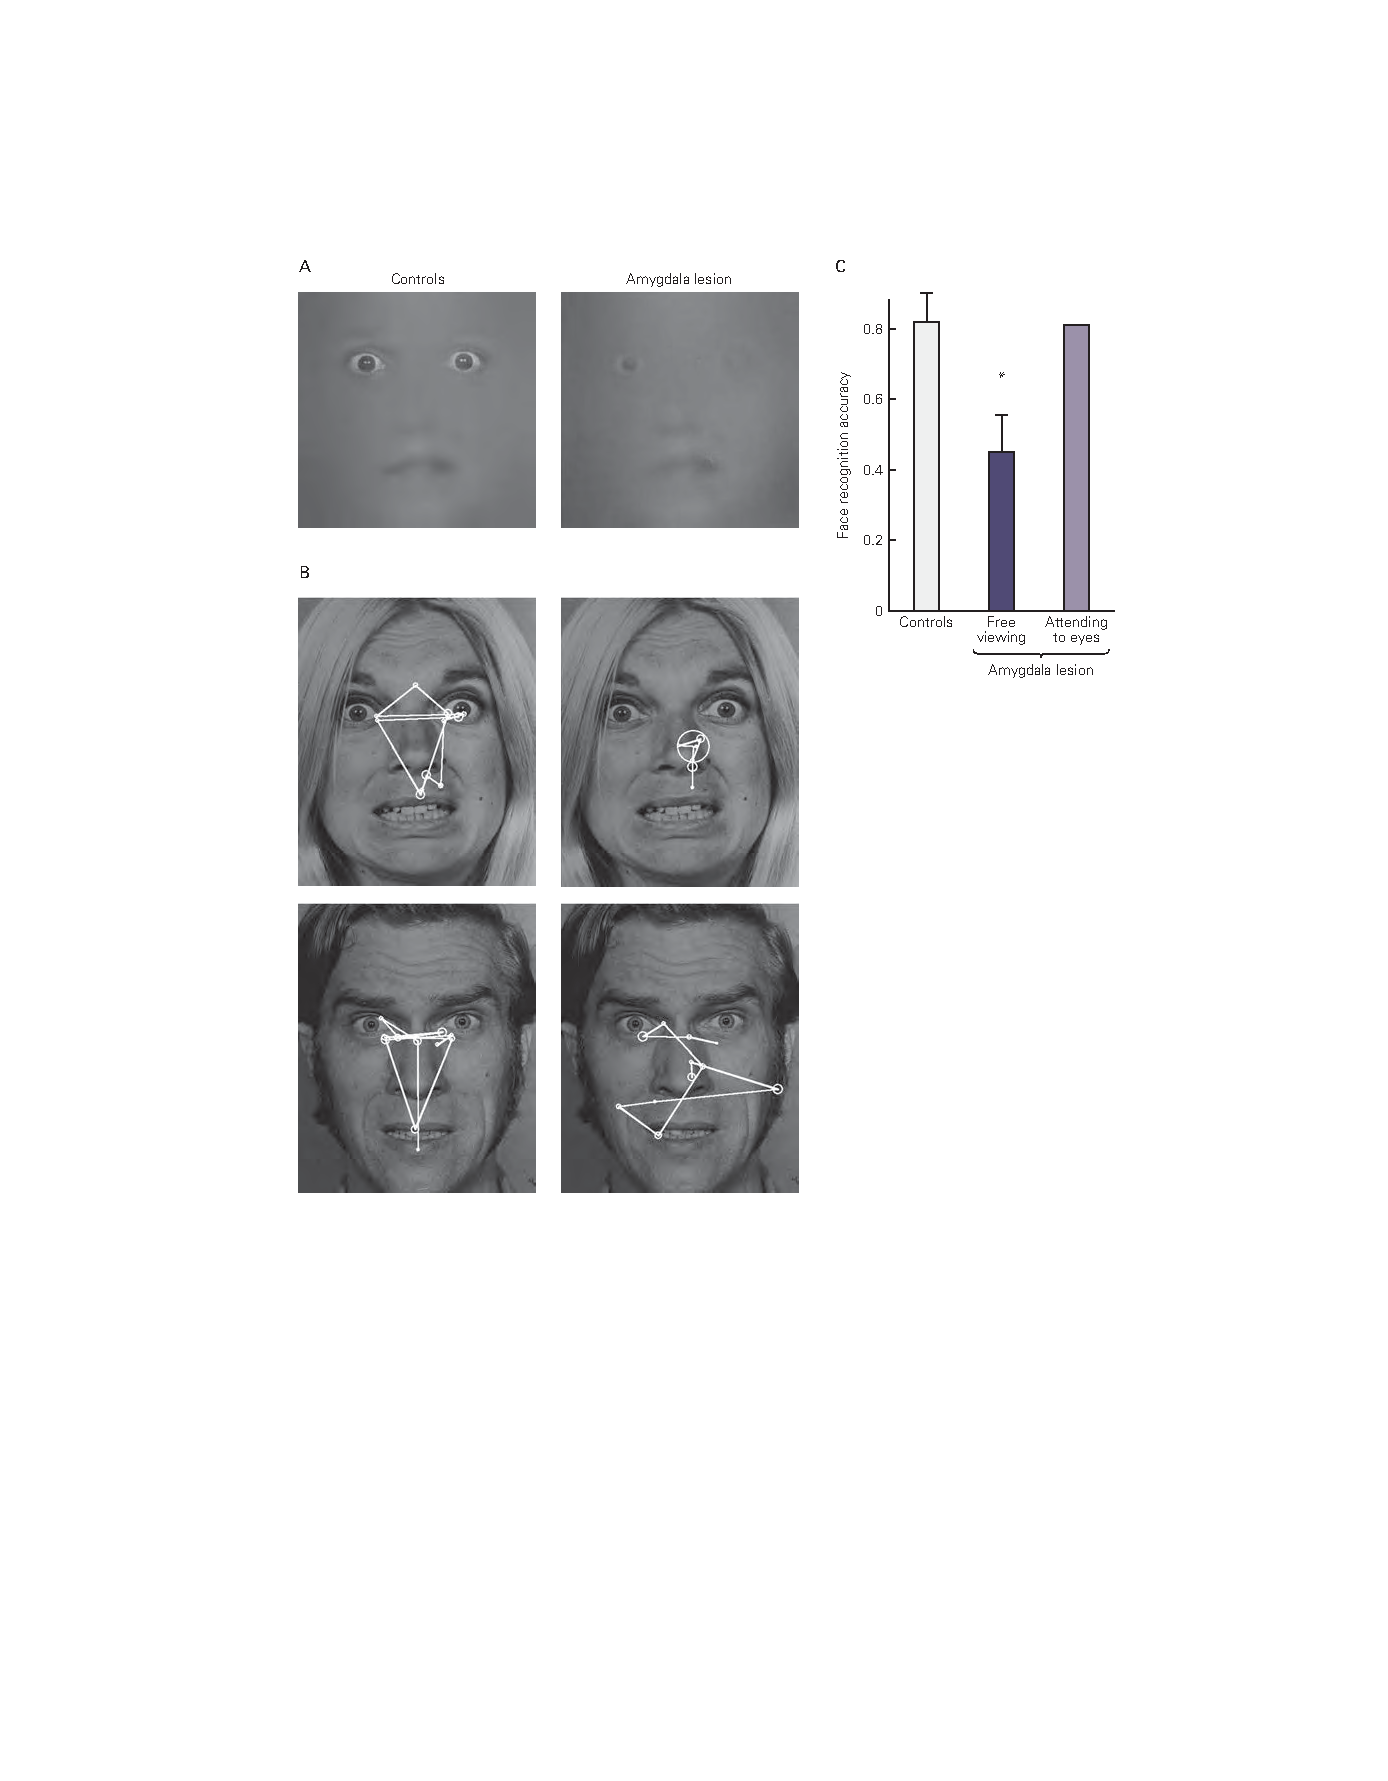
\includegraphics[width=0.75\linewidth]{chap42/fig_42_7}
	\caption{双侧杏仁核损伤会损害他人面部表情中对恐惧的识别。 这种损伤可能是由于对面部信息的异常处理。 (经许可转载自 Adolphs 等人,2005 年。)A. S.M. 在判断情绪时,明显较少使用面部眼部区域的信息。 这些图像显示了控制对象(左)或 S.M. 的面部区域。 (右)能够识别恐惧。 结果是通过向受试者展示许多只露出面部一小部分的试验而获得的。 所有那些受试者能够识别恐惧的试验都可以加起来产生这样的图像,它显示了观众用来区分恐惧和快乐面孔的面部区域(面部的这些特定部分允许 观众区分恐惧和快乐的面孔,而其他部分无助于这种区分)。 B. 在观察整张脸时,S.M. (右)表现出异常的面部凝视(用白线表示),与对照组(左)相比,对眼睛的注视要少得多。 这表明 S.M. 未能注意并因此处理来自眼睛区域的视觉信息。 在所有情绪中都观察到这种缺陷,但对于恐惧识别最为重要,因为睁大眼睛通常预示着恐惧。 C.S.M. 自由观察整张脸(自由观察)时表现出较差的恐惧识别能力,但在被指示看眼睛(注意眼睛)时,她的表现显着提高。 这一结果表明,杏仁核在处理恐惧表情中的作用涉及将注意力引导到特别重要的特征(眼睛)上,而不是解释感官输入的下游过程。}
	\label{fig:42_7}
\end{figure}


这些发现表明杏仁核在注意力方面的重要作用,并强调了某些情绪(如恐惧)的明显特定缺陷可能源于更基本的注意力或动机影响。
关于人类杏仁核在情绪处理的注意力方面的确切作用一直存在争论:一些研究认为它甚至在无意识的威胁相关刺激中以非常自动的方式发挥作用;
其他研究认为,一旦注意力已经分配,杏仁核就需要更精细和有意识的处理。
来自人类杏仁核的单神经元记录支持后一种观点,而一些\textit{功能性磁共振成像}研究支持前一种观点。
人类病变研究的所有发现都需要更精细地剖析;
最近对仅对特定杏仁核亚核有损伤的患者进行的一些研究正在产生进一步的见解。



\section{许多其他大脑区域有助于情绪处理}

正如在条件性和非条件性恐惧的情况下所见,杏仁核作为更大回路或一组回路的一部分有助于情绪处理,该回路包括下丘脑和脑干区域,例如脑干中的导水管周围灰色区域。
皮层区也是该回路的重要组成部分。


许多人类研究表明前扣带皮层、岛叶皮层和腹内侧前额叶皮层的腹侧区域与情绪处理的各个方面有关。
内侧前额叶皮层和杏仁核彼此紧密相连,这些大脑区域的神经元表现出复杂的反应,这些反应编码了许多情绪和认知变量的信息。
这些发现有助于形成情绪状态的动态神经基质的新图景:个体状态不是单一结构或特定神经元的结果,而是更灵活地组装在分布式多功能神经元群中。


有些情绪与社交互动有关,范围从同理心和骄傲到尴尬和内疚。
与恐惧、快乐或悲伤等基本情绪一样,这些社会情绪会产生各种身体变化和行为,并且可以有意识地体验为不同的感受。
这类情绪可能尤其取决于前额叶皮层中的皮层区域。


对神经系统疾病和局灶性脑损伤患者的研究促进了对情绪神经回路的理解(方框 42-2)。
例如,前额叶皮层某些区域的损伤会显着损害社交情绪和相关感受。
此外,这些患者在社交行为方面表现出明显的变化,类似于具有发展性反社会人格的患者的行为。
前额叶皮层部分区域受损的患者无法保住工作,无法维持稳定的社会关系,容易违反社会习俗,无法保持经济独立。
在这种情况发生后,家庭关系和友谊破裂是很常见的。
最近的研究表明,在受控实验条件下,这些患者的道德判断也可能存在缺陷。


与更多背侧或外侧额叶损伤的患者不同,内侧和腹侧额叶损伤的患者没有肢体麻痹或语言障碍等运动缺陷,因此起初可能在神经系统上看起来是正常的。
他们的感知能力、注意力、学习、回忆、语言和运动能力通常没有任何障碍迹象。
一些患者的智商得分处于较高范围。
由于这些原因,他们有时会在脑损伤初步康复后尝试重返工作和社交活动。
只有当他们开始与他人互动时,他们的缺陷才会被发现。


在前额叶皮层中,腹内侧区对于此类相互作用尤为重要。 在大多数社交情绪受损的患者中,该部分双侧受损,尽管仅限于右侧的损伤足以造成损伤。
关键区域包括 Brodmann 区 12、11、10、25 和 32,这些区域接收来自前额皮质背外侧和背内侧区的广泛投射。
其中一些区域广泛投射到与情绪相关的皮层下区域:杏仁核、下丘脑和脑干中的导水管周围灰色区域。


有趣的是,当被问及惩罚、奖励或责任时,腹内侧前额叶皮层受损的成年患者通常会做出反应,就好像他们仍然掌握规则的基本知识,但他们的行为表明他们没有在现实生活中运用这些规则。
这种分离表明,他们的行为缺陷不是由于事实知识的丧失引起的,而是由于大脑将动机价值分配给通常对行为施加控制的因素的分配受损。
在某些方面,这种分离类似于海马体和杏仁核显性和隐性情绪学习之间的分离。
从这些分离中产生的一个有趣的假设是,在其他物种或儿童中,与情绪相关的结构(如杏仁核或腹内侧前额叶皮层)受损后可能会发现更大的缺陷,在这些儿童中,明确的行为控制尚未进化或发展到 它在成人中的程度。
这个想法有一些支持:与成年期持续损伤相比,生命早期这些结构的损伤会导致更严重的情绪和社会行为缺陷(与大多数其他损伤相反的模式,后者显示出更好的恢复) 发病越早发挥作用)。
这些发现还提出了神经功能障碍的假设,这些假设可能导致发育性精神疾病(如自闭症)中出现的情绪困难。


上述病变研究得到了使用功能性核磁共振成像的对照实验研究的补充,这提供了对机制的进一步洞察。
健康人类受试者基于价值的决策的功能成像显示,在做出选择之前的这段时间,腹内侧前额叶皮层被激活。
同样的区域也被惩罚和奖励的管理激活,支持这样一种观点,即预期惩罚和奖励的情感意义被计算为指导这种决策的机制的一部分。
惩罚和奖励经常出现在涉及经济和道德决策的实验中,而此类决策的制定主要涉及许多也涉及处理情绪的相同结构。


前额叶皮层,尤其是腹内侧区,与杏仁核平行运作。
在情绪反应期间,腹内侧区域控制对特定刺激的注意力,影响从记忆中检索的内容,并帮助形成对触发刺激做出反应的心理计划。
通过影响注意力,杏仁核和腹内侧前额叶皮层也可能改变认知过程,例如,通过加快或减慢感觉表征的流动(第~\ref{chap:chap17}~章)。



\section{功能性神经影像学有助于我们理解人类的情绪}

情绪的神经影像学研究通常使用功能性核磁共振成像。 这些研究在三个重要方面促进了我们对情绪的理解。
首先,他们已经开始分离和实验性地操纵情绪的特定方面,例如感觉、价值或情绪概念。
这些研究开始表明所有这些不同方面如何通过不同大脑区域的活动进行协调。


其次,关于情绪的功能性核磁共振成像研究一直在以越来越快的速度积累,这些研究的大部分数据现在都可以广泛获得。
这为许多研究的荟萃分析提供了机会,避免了任何一项孤立的研究可能固有的局限性。
例如,一些荟萃分析证实了腹内侧前额叶皮层在代表许多不同类型刺激(包括食物和金钱)的价值方面的作用。
其他荟萃分析表明,特定的基本情绪(例如,恐惧、愤怒或快乐)会激活一组广泛分布且重叠的大脑区域,从而证实了没有大脑结构负责单一情绪的观点。


最后,功能性核磁共振成像研究已经开始在他们的分析中使用新方法。
例如,在一个大脑区域的许多体素中看到的激活模式,而不是该区域的平均激活水平,被用来训练强大的机器学习算法来对情绪状态进行分类。
这种方法表明,可以从大脑激活的分布式模式中解码特定的情绪状态。



\subsection{功能成像已经确定了感觉的神经相关性}

对情绪的有意识体验通常被称为感觉。
感觉的神经相关性的证据主要来自人类的功能成像研究和特定脑损伤患者的神经心理学测试。
这些研究的一个主要挑战是将情绪的有意识体验与情绪的其他方面分离,例如生理反应的诱发,因为这些往往同时发生。
另一个挑战是如何将此类研究与动物情绪研究联系起来,我们没有商定的依赖措施来分析他们有意识的体验。


一项早期的功能成像研究使用正电子发射断层扫描来检验这样一种观点,即感觉与皮质和皮质下体感区域的活动相关,这些区域专门接收与内部环境(内脏、内分泌腺和肌肉骨骼系统)相关的输入。
要求健康受试者回忆个人事件,并尝试尽可能重新体验伴随这些事件的情绪。
许多已知代表和调节身体状态的区域的活动发生了变化,例如岛叶皮层、次级体感皮层 (S-II)、扣带皮层、下丘脑和上脑干。
这些结果支持这样一种观点,即感觉的神经基质至少有一部分涉及调节和代表身体状态的大脑区域,这一发现与前面提到的 William James 的假设有些相似,即感觉是基于对身体的意识 反应。


最近的功能性核磁共振成像研究也证实了皮层和皮层下结构在处理感觉中的重要性。
其中一项研究检查了预期电击引起的恐惧感(图~\ref{fig:42_8})。
在这项研究中,受试者躺在扫描仪中,同时他们在视频屏幕上看到一个游戏,其中一个虚拟捕食者(一个红点)离受试者越来越近。
一旦捕食者抓住了它们,它们的手就会受到痛苦的电击。
当捕食者远离一定距离时产生的焦虑与内侧前额叶皮层的激活有关;
当捕食者靠近时,导水管周围的灰色被激活,这与受试者报告的恐惧感相关。
这一发现支持内侧前额叶皮层在与远距离威胁相关的计划和预期中的作用,以及导水管周围灰质在建立应对直接威胁所需的防御反应中的作用。


\begin{figure}[htbp]
	\centering
	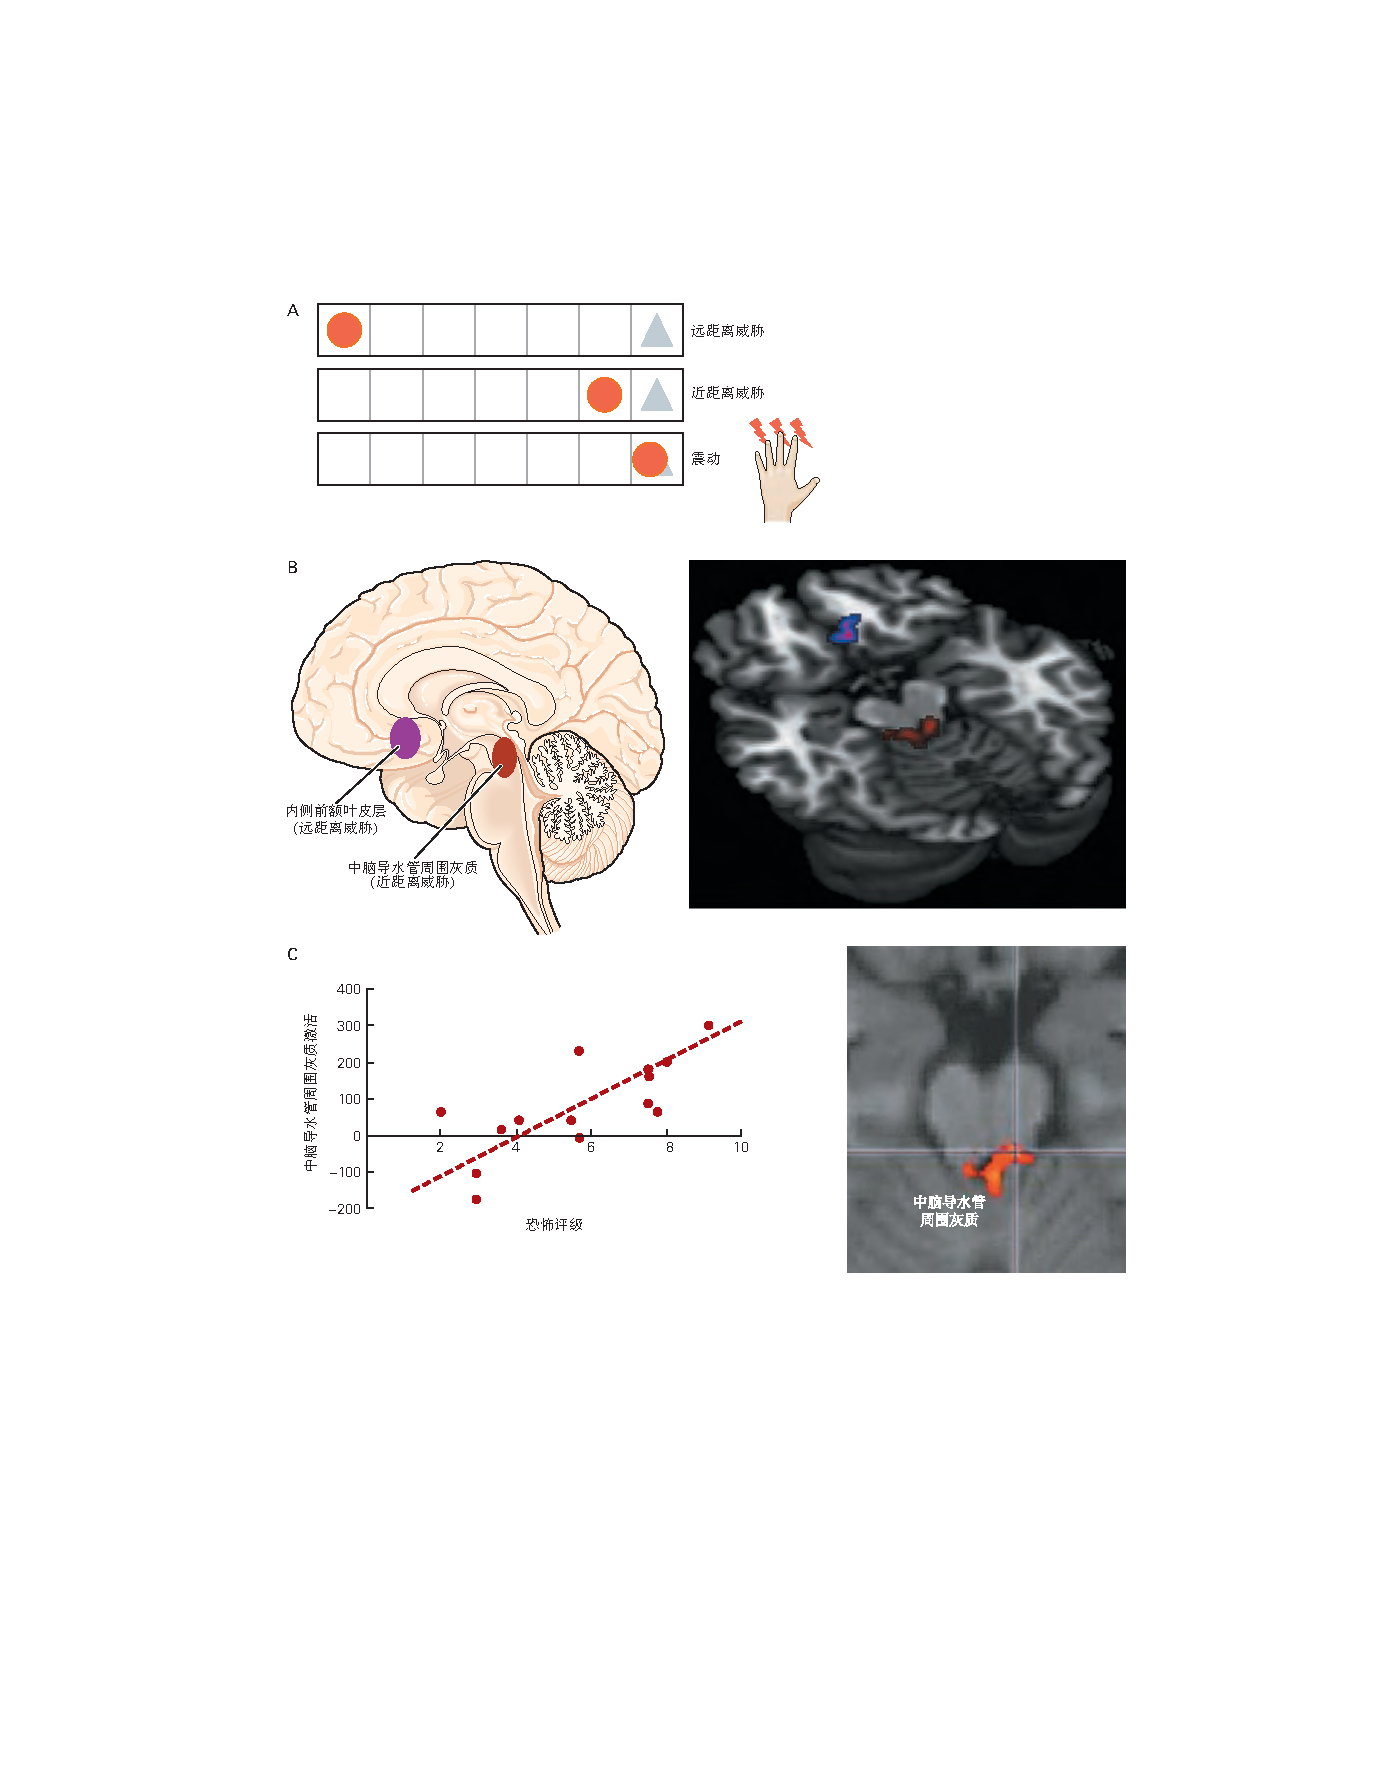
\includegraphics[width=0.75\linewidth]{chap42/fig_42_8}
	\caption{皮质和皮质下区域都会在情绪状态下发挥作用。 结果来自功能性磁共振成像研究,其中受试者躺在扫描仪中,同时观察虚拟捕食者(红点)在屏幕上四处移动并靠近受试者(蓝色三角形,代表实际研究参与者)。 (经许可转载自 Mobbs 等人,2007 年。版权所有 © 2007 AAAS。) A. 一旦捕食者追上目标,手部就有可能受到真实而痛苦的电击。 B. 当捕食者靠近主体时,前额叶皮层和导水管周围灰质的活动增加。 值得注意的是,这种神经激活模式发生了变化,使得远处的捕食者在内侧前额叶皮层引起更多活动,而靠近的捕食者在导水管周围灰质中引起更多活动。 C. 导水管周围灰质 (PAG) 的激活与主体在扫描仪中给出的评分所衡量的主观恐惧感相关。}
	\label{fig:42_8}
\end{figure}


另一个与感觉相关的大脑区域是前扣带皮层的膝下区(Brodmann 区 25),在神经影像学研究中发现,当受试者感到悲伤时,它会被激活。
该区域特别令人感兴趣,因为它在双相抑郁症患者中也有差异激活,并且在慢性抑郁症患者的结构核磁共振成像扫描中显得变薄。
对这个大脑区域进行直接电刺激(深部脑刺激)可以显着改善一些严重抑郁症患者的情绪。



\subsection{情绪与体内平衡有关}

虽然很明显没有大脑区域专门负责任何特定的情绪,但是否存在专门负责一般情绪的大脑区域甚至值得怀疑。
可能涉及情绪的所有大脑区域也执行其他功能。
事实上,这些非情绪功能可能会为我们提供有关情绪如何演变的线索,而且实际上可能是情绪状态组装的基本构件。


例如,在回忆感觉时被激活的人类岛叶皮层部分在有意识的疼痛和温度感觉时也会被激活。
岛叶皮层通过起源于周围神经纤维的通路接收稳态信息(关于温度和疼痛、血液 pH 值、二氧化碳和氧气的变化)。
这些传入纤维包括,例如,与脊髓后角 I 层或脑干三叉神经核尾部的神经元形成突触的 C 和 Aδ 纤维。
从椎板 I 和三叉神经核投射到脑干核团(孤束核和臂旁核)的通路,然后从那里投射到丘脑和岛叶皮层。
该功能系统的识别进一步支持了传入体感通路中的信号在感觉处理中发挥作用的观点。


此外,在纯自主神经功能衰竭患者中,一种内脏传入信息严重受损的疾病,功能成像研究显示情绪过程迟钝,体感区域活动减弱,这些区域有助于感受。
与其他感受一样,社会感受涉及岛叶皮层以及初级和次级体感皮层(S-I 和 S-II),正如在评估对疼痛的同理心以及单独的钦佩和同情心的功能性神经影像学实验中发现的那样。


使用这些数据作为支持,一些有影响力的现代理论建立在 William James 最初的假设之上,并提出所有情绪的感觉都基于大脑对身体稳态的表征。
正如杏仁核在积极和消极情绪中的作用一样,脑岛在处理内感受和情绪信息中的作用仍然与这些过程不同的可能性相一致。
也就是说,这些结构中的不同神经元群可能参与处理不同的情绪。
因此,功能性核磁共振成像可能无法提供阐明不同但解剖学上混合的神经元群体所需的分辨率水平,并且可能需要动物模型中的细胞技术。


尽管迄今为止大多数神经科学研究都集中在消极情绪上,但在人类和动物身上的研究正在阐明积极情绪的神经回路。
这些研究一致认为内侧前额叶皮层参与计算奖励的主观价值,伏隔核和基底神经节的其他核参与处理积极情绪的享乐成分(或快乐)。
越来越多的人类功能成像研究——尤其是在神经经济学和社会神经科学领域——将这些结构在情绪处理中的作用与其在基于价值的决策制定和社会行为中的作用联系起来。



\section{要点}

1. 在调节生物体的身体和行为的整体生理学中,情绪状态一方面发挥着与更简单的反射和稳态调节过程以及另一方面的认知过程和故意行为的中间过程的功能。
情绪比简单的反射更灵活、更依赖于情境和可控,但不如有意的行为更灵活、更依赖于情境和更受控。
情绪演变为响应反复出现的环境和内部挑战而产生的行为,这些挑战对于反应来说过于多样化,但足够刻板以至于它们不需要认知的充分灵活性。


2. 需要将情绪状态与有意识的情绪体验(感觉)以及我们在日常语言中用来描述情绪的概念和词语仔细区分开来。
例如,一只发出嘶嘶声的猫的行为是由情绪状态引起的,但猫是否有意识地感到害怕尚不清楚。
猫可能没有概念,当然也没有语言来思考这种情绪。
在观察面部表情时识别出恐惧的人类受试者将恐惧归因于另一个人并且正在思考特定的情绪,但他们自己不一定处于恐惧状态或经历恐惧。
独立控制和操纵情绪的这些不同成分是设计实验的主要挑战,尤其是在人类实验中。


3. 情绪协调许多有机体参数的综合变化,包括对躯体行为、自主神经和内分泌反应以及认知的影响。
我们尚不了解这种协调是如何产生的,尽管它可能是通过分层控制(通过充当各种“指挥中心”的大脑区域)和分布式动力学的组合来实现的。
了解这是如何在生物有机体中完成的,也将为我们如何设计未来表现出情感行为的机器人提供信息。


4. 不同的特定情绪可以分类(例如快乐、恐惧、愤怒)或维度(根据唤醒和效价或其他维度框架)来思考。
一旦我们有了更科学的理解,许多我们有特定语言单词的类别(如刚刚给出的例子)很可能需要修改。
应用于使用功能性核磁共振成像获取的数据的新分析方法,包括考虑大脑活动的空间和时间模式并利用强大的机器学习算法的方法,可以为大脑如何调节广泛的情绪提供新的见解。


5. 在人类中,情绪可以通过多种机制进行调节。
因此,我们可以控制自己的感受,也可以控制表达情绪行为的方式,例如通过面部表情。
非人类动物没有这种相同水平的控制,因此它们的情绪行为通常是它们情绪状态的诚实信号,而人类则经常进行策略欺骗。


6. 恐惧可能是神经生物学最好理解的情绪。
这取决于动物和人类的杏仁核。
然而,一些数据表明某些类型的恐惧,例如吸入二氧化碳引起的窒息恐慌,与杏仁核无关。
事实上,我们现在知道杏仁核是分布式大脑系统的一部分,因此,许多其他大脑区域也参与处理恐惧。
现代研究越来越多地使用复杂的遗传和细胞技术来成像和因果操纵大脑功能,使我们能够理解多个大脑结构在调节不同情绪行为中的必要和充分作用。


7. 腹侧和内侧前额叶皮层与情绪密切相关,并与杏仁核相连。
社会情绪、奖励表征、情绪调节和消退都涉及前额叶皮层的特定区域。
大脑的这个区域,连同脑岛,对于我们有意识的情绪体验也可能是最重要的,情绪的一个方面仍然是最具挑战性的研究。

